%-----------------------------------------------------------------------------------
%   PACKAGES 
%-----------------------------------------------------------------------------------

\documentclass[a4paper,11pt,abstracton]{scrartcl}

\usepackage[margin=.9in]{geometry}


\usepackage{mlmodern}


\usepackage{amsmath,amsthm,amssymb}
\usepackage{mathtools,mathrsfs}
\usepackage{centernot}
\usepackage{wrapfig}

\usepackage{tikz,tikz-cd,asymptote}
\usetikzlibrary{positioning, fit, calc}

\usepackage[most]{tcolorbox}
\usepackage{hyperref,wrapfig}
\usepackage[dvipsnames]{xcolor}
\usepackage{enumerate}
\usepackage[a]{esvect}
\usepackage{tocloft}


\usepackage{sectsty}
\makeatletter
\def\@seccntformat#1{\textcolor{Red}{\hspace*{0.2em}$\textbf{\S}$\hspace{-0.3em} \csname the#1\endcsname}\hspace{0.5em}}
\makeatother

\usepackage{fancyhdr}
\pagestyle{fancy}
\lhead{Elementary Number Theory}
\rhead{\thepage}
\cfoot{} 

\setlength{\parindent}{0cm}

%-----------------------------------------------------------------------------------
%   COMMANDS
%-----------------------------------------------------------------------------------

\DeclarePairedDelimiter{\floor}{\lfloor}{\rfloor}

\newcommand{\nonadj}{\,\neg\textsf{adj}\,}
\newcommand{\adj}{\,\textsf{adj}\,}
\newcommand{\RR}{\mathbb{R}}
\newcommand{\ZZ}{\mathbb{Z}}
\newcommand{\NN}{\mathbb{N}}
\newcommand{\CC}{\mathbb{C}}
\newcommand{\QQ}{\mathbb{Q}}
\newcommand{\sgn}{\text{sgn\hspace{0.5mm}}}
\newcommand{\osc}{\text{osc\hspace{0.5mm}}}
\newcommand{\foralls}{\hspace{2mm}\forall}
\newcommand{\rimply}{\Rightarrow}
\newcommand{\limply}{\Leftarrow}
\newcommand{\underdash}{\rule{0.25cm}{0.1mm}\hspace{0.5mm}}
\newcommand{\undersmalldash}{\rule{0.18cm}{0.1mm}\hspace{0.3mm}}
\newcommand{\s}{\square}
\newcommand{\xr}{\xrightarrow}

\newcommand{\genstirlingI}[3]{%
  \genfrac{[}{]}{0pt}{#1}{#2}{#3}%
}
\newcommand{\genstirlingII}[3]{%
  \genfrac{\{}{\}}{0pt}{#1}{#2}{#3}%
}
\newcommand{\genlah}[3]{%
  \genfrac{\lfloor}{\rfloor}{0pt}{#1}{#2}{#3}%
}
\newcommand{\stirlingI}[2]{\genstirlingI{}{#1}{#2}}
\newcommand{\stirlingII}[2]{\genstirlingII{}{#1}{#2}}
\newcommand{\lah}[2]{\genlah{}{#1}{#2}}

%-----------------------------------------------------------------------------------
%   ENVIROMENTS
%-----------------------------------------------------------------------------------

\newtheoremstyle{dotlessP}{}{}{}{}{\color{RedViolet}\bfseries}{.}{ }{}
\theoremstyle{dotlessP}
\newtheorem{problem}{Problem}
\newtheoremstyle{dotlessS}{}{}{}{}{\color{ForestGreen}\bfseries}{.}{ }{}
\theoremstyle{dotlessS}
\newtheorem*{solution}{Solution}

\theoremstyle{remark}
\newtheorem*{remark}{Remark}
\theoremstyle{definition}
\newtheorem*{theorem}{Theorem}

\tcbset {
  base/.style={
    arc=0mm, 
    bottomtitle=0.5mm,
    boxrule=0mm,
    colbacktitle=black!10!white, 
    coltitle=black, 
    fonttitle=\bfseries, 
    left=2.5mm,
    leftrule=1mm,
    right=3.5mm,
    title={#1},
    toptitle=0.75mm, 
  }
}

\definecolor{brandblue}{rgb}{0.34, 0.7, 1}

\newtcolorbox{mainbox}[1]{
  enhanced jigsaw,
  breakable,
  colframe=brandblue, 
  base={#1}
}

\newtcolorbox{subbox}[1]{
  colframe=black!30!white,
  base={#1}
}

\newtcolorbox{definition_box}{
enhanced jigsaw,
breakable,
pad at break*=1mm,
colback=lightgray!12!white,
colframe=RedViolet!45!black,
colbacktitle=Gray!38!white,
before={\vspace{4mm}},
after={\vspace{2mm}},
sharp corners
}


\newtcolorbox{problem_box}{
enhanced jigsaw,
breakable,
pad at break*=1mm,
colback=white!5!white,
colframe=gray!75!black,
colbacktitle=white!28!white,
sharp corners,
before={\vspace{6mm}},
after={\vspace{2mm}}
}

\newtcolorbox{problem_box_1}{
enhanced jigsaw,
breakable,
pad at break*=1mm,
colback=SeaGreen!5!white,
colframe=SeaGreen!75!black,
colbacktitle=Black!28!white,
sharp corners,
before={\vspace{6mm}},
after={\vspace{2mm}}
}

\newtcolorbox{problem_box_title}[1]{
enhanced jigsaw,
breakable,
pad at break*=1mm,
colback=Apricot!5!white,
colframe=Melon!75!black,
sharp corners,
before={\vspace{2mm}},
after={\vspace{2mm}},
title={#1}, 
fonttitle=\bfseries
}

\newtcolorbox{claim_box}{
enhanced jigsaw,
breakable,
pad at break*=1mm,
colback=white,
colframe=white,
borderline west={2pt}{0pt}{white},
sharp corners,
before={\vspace{1mm}},
after={\vspace{0.8mm}}
}

\newtcolorbox{example_box}{
enhanced jigsaw,
breakable,
pad at break*=1mm,
colback=lightgray!12!white,
colframe=lightgray!15!white,
borderline west={2pt}{0pt}{black},
sharp corners,
before={\vspace{2mm}},
after={\vspace{2mm}}
}

\newtcolorbox{remark_box}{
enhanced jigsaw,
breakable,
pad at break*=1mm,
colback=Apricot!5!white,
colframe=Melon!75!black,
sharp corners,
before={\vspace{2mm}},
after={\vspace{2mm}}
}


\begin{document}

%-----------------------------------------------------------------------------------
%   TOP MATTERS
%-----------------------------------------------------------------------------------

\title{Elementary Number Theory}
\subtitle{Handkerchief}
\author{Pratyay Sen}
\date{September 29, 2026}
\maketitle

\tableofcontents

\eject


%-----------------------------------------------------------------------------------
%   MAIN BODY
%-----------------------------------------------------------------------------------

\section{Well-Ordering and Mathematical Induction}

We begin with two equivalent principles that underlie many proofs in
number theory. It would not be an exaggeration to say that the entire branch of number theory would not exist without these two. Another interesting fact is that both of these are equivalent to one of my favourite axioms, the Axiom of Choice (more on that in the set theory section of this book). Let us first see what these two principles are, and how they are equivalent. Throughout this section, let
$\mathbb{N}_0=\{0,1,2,\ldots\}$.

\begin{definition_box}
\textbf{Well-ordering principle:}
Every nonempty subset $S\subseteq\mathbb{N}_0$ has a least element:
there is an $m\in S$ such that $m\leq s$ for every $s\in S$.
\end{definition_box}

\begin{definition_box}
\textbf{Principle of mathematical induction:}
Let $P(n)$ be a statement about $n\in\mathbb{N}_0$. If
\begin{enumerate}
    \item $P(0)$ holds (the \emph{base case}), and
    \item for every $k\in\mathbb{N}_0$, $P(k)$ implies $P(k+1)$
    (the \emph{inductive step}),
\end{enumerate}
then $P(n)$ holds for every $n\in\mathbb{N}_0$.
\end{definition_box}

\begin{mainbox}{Theorem:}
The well-ordering principle and the principle of mathematical induction
are equivalent.
\end{mainbox}

\subsection{Well-Ordering Implies Induction}

Suppose the well-ordering principle holds, and let $P(n)$ satisfy the
base case and inductive step. Assume, for a contradiction, that $P(n)$
is false for at least one nonnegative integer. Then the set of
counterexamples
\[
    C=\{n\in\mathbb{N}_0 : P(n)\text{ is false}\}
\]
is nonempty, so it has a least element $m$. Since $P(0)$ is true,
$m\neq0$, and hence $m-1\in\mathbb{N}_0$. Minimality of $m$ implies
that $P(m-1)$ is true. The inductive step now gives $P(m)$, contradicting
$m\in C$. Thus there are no counterexamples, and $P(n)$ holds for every
$n\in\mathbb{N}_0$.
\hfill$\square$

\subsection{Induction Implies Well-Ordering}

Suppose the principle of mathematical induction holds. Let
$S\subseteq\mathbb{N}_0$ be nonempty, and assume, for a contradiction,
that $S$ has no least element. Consider the statement
\[
    Q(n):\qquad S\cap\{0,1,\ldots,n\}=\varnothing.
\]
We prove $Q(n)$ by induction.

\textit{Base case:}
If $0\in S$, then $0$ would be its least element. Hence $0\notin S$,
so $Q(0)$ holds.

\textit{Inductive step:}
Assume $Q(k)$ holds. If $k+1\in S$, then, since none of
$0,1,\ldots,k$ belongs to $S$, the integer $k+1$ would be the least
element of $S$. This contradicts our assumption. Therefore $k+1\notin S$,
and $Q(k+1)$ holds.

By induction, $Q(n)$ holds for every $n\in\mathbb{N}_0$. But choosing
any $s\in S$ contradicts $Q(s)$. Thus $S$ must have a least element,
which proves the well-ordering principle.
\hfill$\square$

\subsection{Strong Induction}

\begin{definition_box}
An equivalent version of induction, is
\emph{strong induction}: if $P(0)$ holds and, for every $k\geq0$,
\[
    P(0),P(1),\ldots,P(k)\quad\Longrightarrow\quad P(k+1),
\]
then $P(n)$ holds for every $n\in\mathbb{N}_0$.
\end{definition_box}

Ordinary induction proves this by applying it to the cumulative statement
$R(n)$ that $P(j)$ holds for every $0\leq j\leq n$.
Conversely, an ordinary inductive step is a special case of a strong
inductive step, since the latter includes $P(k)$ among its assumptions.
Thus well-ordering, ordinary induction, and strong induction are
interchangeable proof principles. All of these are very useful in number theory for proving a variety of results.

\section{Divisibility}

Divisibility sits at the very core of number theory, because the very notion of a number dividing another gave birth to modular arithmetic, the concept of primes, and basically the entirety of number theory.

\begin{definition_box}
For integers $a$ and $b$, we write $a\mid b$ if there exists an integer
$k$ such that $b=ak$.
\end{definition_box}

\begin{example_box}
For example, $7\mid 42$, but $7\nmid 45$.
\end{example_box}

\begin{remark_box}
If $a\mid b$ and $a\mid c$, then
\[
    a\mid (ub+vc)\qquad\text{for every }u,v\in\mathbb{Z}.
\]
\end{remark_box}

\textbf{Proof:}
Since $a\mid b$ and $a\mid c$, there exist integers $r,s$ such that
$b=ar$ and $c=as$. For any integers $u,v$, we therefore have
\[
    ub+vc=u(ar)+v(as)=a(ur+vs).
\]
Because $ur+vs\in\mathbb{Z}$, the definition of divisibility gives
$a\mid(ub+vc)$.
\hfill$\square$


\begin{remark_box}
The division algorithm states that for every integer $a$ and positive
integer $b$, there are unique integers $q,r$ with
\[
    a=bq+r,\qquad 0\leq r<b.
\]
\end{remark_box}

\textbf{Proof of existence:}
Consider the set of nonnegative candidate remainders
\[
    S=\{a-bk : k\in\mathbb{Z},\ a-bk\geq0\}.
\]
This set is nonempty: taking $k=-|a|$ gives
$a+b|a|\geq a+|a|\geq0$, since $b\geq1$.
By the well-ordering principle, $S$ has a least element $r$.
By definition of $S$, there is an integer $q$ with $r=a-bq$, so
$a=bq+r$ and $r\geq0$.

If $r\geq b$, then
\[
    r-b=a-b(q+1)\geq0,
\]
so $r-b$ would also belong to $S$. But $b>0$ implies $r-b<r$,
contradicting the minimality of $r$. Therefore $0\leq r<b$.


\textbf{Proof of uniqueness:}
Suppose there are two representations
\[
    a=bq+r=bq'+r',\qquad 0\leq r,r'<b.
\]
Subtracting yields
\[
    b(q-q')=r'-r.
\]
Since $-b<r'-r<b$, the integer $r'-r$ is a multiple of $b$ with
absolute value strictly less than $b$. The only such multiple is $0$.
Thus $r'=r$, and then $b(q-q')=0$ gives $q=q'$ because $b>0$.
This proves both existence and uniqueness, including when $a$ is negative.
\hfill$\square$

We'll be using well ordering, induction and divisibility throughout this section, so make sure you remember them!! (or write them in a piece of paper)

\section{GCD and LCM}

After looking at divisibility, a natural question one might ask is what about the common divisors of two numbers? Or the common multiples? It is obvious that the lowest common divisor for any two numbers is 1, and the greatest common multiple is infinity. Therefore, it makes sense to talk about the greatest common divisor and least common multiple.

\subsection{Greatest Common Divisors}

\begin{definition_box}
For integers $a,b$ that are not both zero, their greatest common divisor,
written $\gcd(a,b)$, is the largest positive integer dividing both.
\end{definition_box}

\begin{definition_box}
If $\gcd(a,b)=1$, we say that $a$ and $b$ are \emph{coprime} or \emph{relatively prime}.
\end{definition_box}

Euclid had developed a very useful algorithm in order to find the gcd of any two numbers, because prime factorisation is not a suitable method all the time.

\begin{mainbox}{Euclidean Algorithm}
For integers $a,b$ not both zero, repeated division computes
$\gcd(a,b)$: the algorithm terminates, and its last nonzero remainder
is the greatest common divisor.
\textit{}
If $a=bq+r$ with $b>0$ and $0\leq r<b$, then
\[
    \gcd(a,b)=\gcd(b,r).
\]
Indeed, any common divisor of $a,b$ divides $r=a-bq$. Conversely,
any common divisor of $b,r$ divides $a=bq+r$. Thus the two pairs
have exactly the same positive common divisors, and hence the same gcd.
\end{mainbox}

\begin{subbox}{Procedure}
Replace the inputs by their absolute values and, if necessary, interchange
them so that $r_0\geq r_1\geq0$, with $r_0>0$.
These operations do not change the gcd. If $r_1=0$, return $r_0$,
since $\gcd(r_0,0)=r_0$. Otherwise, repeatedly apply the division
algorithm:
\[
    r_{j-1}=q_jr_j+r_{j+1},\qquad 0\leq r_{j+1}<r_j,
\]
for $j=1,2,\ldots$, stopping as soon as $r_{j+1}=0$.
\end{subbox}

\textbf{Proof of termination:}
If the procedure never stopped, it would produce an infinite strictly
decreasing sequence of positive integers
\[
    r_1>r_2>r_3>\cdots.
\]
By well-ordering, the set of these remainders would have a least element
$r_k$. But the next remainder $r_{k+1}$ would be positive and smaller
than $r_k$, a contradiction. Therefore, for some $n\geq1$, we reach
$r_n>0$ and $r_{n+1}=0$.


\textbf{Proof of correctness:}
The basic step preserves the gcd at every division. Hence
\[
    \gcd(a,b)=\gcd(r_0,r_1)
    =\gcd(r_1,r_2)=\cdots
    =\gcd(r_n,r_{n+1})=\gcd(r_n,0)=r_n.
\]
Thus the last nonzero remainder is exactly the gcd of the original
inputs.
\hfill$\square$



\begin{example_box}
\textit{Example:}
To find $\gcd(252,105)$, perform the divisions
\begin{align*}
    252&=2\cdot105+42,\\
    105&=2\cdot42+21,\\
    42&=2\cdot21.
\end{align*}
The last nonzero remainder is $21$, so $\gcd(252,105)=21$.
\end{example_box}


\begin{mainbox}{B\'ezout's theorem:}
For integers $a,b$ not both zero, there exist integers $u,v$ such that
\[
    au+bv=\gcd(a,b).
\]
\end{mainbox}

\textbf{Proof:}
Consider the set of positive integer linear combinations of $a$ and $b$,
\[
    S=\{ax+by : x,y\in\mathbb{Z},\ ax+by>0\}.
\]
Since $a,b$ are not both zero, at least one of $|a|$ and $|b|$ is
positive and belongs to $S$. Thus $S$ is nonempty. By well-ordering,
$S$ has a least element $d$, and we may write
\[
    d=au+bv>0
\]
for some integers $u,v$.

Apply the division algorithm to $a$ with divisor $d$:
\[
    a=dq+r,\qquad 0\leq r<d.
\]
Then
\[
    r=a-qd=a(1-qu)+b(-qv).
\]
If $r>0$, this would be an element of $S$ smaller than $d$, a
contradiction. Hence $r=0$, so $d\mid a$.
Likewise, writing $b=dq'+r'$ with $0\leq r'<d$ gives
\[
    r'=b-q'd=a(-q'u)+b(1-q'v).
\]
Minimality again forces $r'=0$, so $d\mid b$.

Finally, every positive common divisor $c$ of $a$ and $b$ divides
$au+bv=d$. Since $c,d>0$, this implies $c\leq d$.
Therefore $d$ is the greatest common divisor of $a$ and $b$, proving
$au+bv=\gcd(a,b)$.
\hfill$\square$



\begin{example_box}
These coefficients can be found by backward substitution in the Euclidean
algorithm. In the example above,
\[
    21=105-2(252-2\cdot105)=-2\cdot252+5\cdot105.
\]
\end{example_box}

Thus begins the barrage of lemmas...

\begin{remark_box}
\textbf{Lemma:}
For integers $a,b$ not both zero,
\[
    \gcd(a,b)=1
    \quad\Longleftrightarrow\quad
    \text{there exist }x,y\in\mathbb{Z}\text{ such that }ax+by=1.
\]
Here $(a,b)$ is another common notation for $\gcd(a,b)$.
The coefficients $x,y$ are required to exist; the equation need not
hold for arbitrary choices of $x,y$.
\end{remark_box}

\textbf{Proof:}
If $\gcd(a,b)=1$, B\'ezout's identity immediately supplies integers
$x,y$ with $ax+by=1$.

Conversely, suppose $ax+by=1$ for some integers $x,y$. Let
$d=\gcd(a,b)$. Since $d\mid a$ and $d\mid b$, we have
$d\mid(ax+by)=1$. As $d$ is positive, $d=1$.
This proves the equivalence.
\hfill$\square$



\begin{example_box}
For example, $3\cdot5-2\cdot7=1$, so $\gcd(5,7)=1$.
\end{example_box}


\begin{remark_box}
\textbf{Lemma:}
Let $a,b$ be integers, not both zero, and let $d=\gcd(a,b)$. Then
\[
    \gcd\!\left(\frac{a}{d},\frac{b}{d}\right)=1.
\]
\end{remark_box}

\textbf{Proof:}
Since $d>0$ divides both $a$ and $b$, the quotients $a/d$ and $b/d$
are integers. By B\'ezout's identity, there exist integers $x,y$ such that
\[
    ax+by=d.
\]
Dividing by $d$ gives
\[
    \frac{a}{d}x+\frac{b}{d}y=1.
\]
The coprimality criterion therefore implies
$\gcd(a/d,b/d)=1$.
\hfill$\square$


\begin{remark_box}
\textbf{Lemma:}
Let $a,b,c$ be integers with $\gcd(a,b)=1$. If $a\mid c$ and
$b\mid c$, then $ab\mid c$.
\end{remark_box}

\textbf{Proof:}
Since $a\mid c$ and $b\mid c$, there exist integers $r,s$ such that
$c=ar=bs$. By B\'ezout's identity, there exist integers $x,y$ with
$ax+by=1$. Multiplying this identity by $c$ gives
\[
    c=axc+byc=ax(bs)+by(ar)=ab(xs+yr).
\]
Since $xs+yr$ is an integer, $ab\mid c$.
\hfill$\square$



\begin{example_box}
\textit{Why the coprimality assumption matters:}
Without $\gcd(a,b)=1$, the conclusion need not hold. For example,
$4\mid12$ and $6\mid12$, but $4\cdot6=24\nmid12$.
\end{example_box}


\begin{remark_box}
\textbf{Euclid's lemma:}
Let $a,b,c,d$ be integers with $\gcd(a,b)=1$. If $ac=bd$, then
$a\mid d$.
\end{remark_box}

\textbf{Proof:}
By B\'ezout's identity, there exist integers $x,y$ such that
$ax+by=1$. Multiplying by $d$ and using $bd=ac$, we obtain
\[
    d=axd+byd=a(xd)+y(bd)=a(xd)+y(ac)=a(xd+cy).
\]
Since $xd+cy$ is an integer, $a\mid d$.
\hfill$\square$


Equivalently, if $\gcd(a,b)=1$ and $a\mid bd$, then $a\mid d$:
the divisibility $a\mid bd$ means precisely that $ac=bd$ for some
integer $c$.

\subsection{Least Common Multiples}

\begin{definition_box}
For positive integers $a,b$, the \emph{least common multiple}, denoted
$\operatorname{lcm}(a,b)$ or $[a,b]$, is the smallest positive integer
that is divisible by both $a$ and $b$.
\end{definition_box}

It exists because the set of
positive common multiples is nonempty (it contains $ab$) and therefore
has a least element by well-ordering. 

\begin{example_box}
For example, $[4,6]=12$ and $[8,9]=72$.
\end{example_box}

\begin{mainbox}{The gcd-lcm identity:}
For positive integers $a,b$,
\[
    ab=\gcd(a,b)\operatorname{lcm}(a,b)=(a,b)[a,b].
\]
\end{mainbox}

\textbf{Proof:}
Let $d=\gcd(a,b)$ and write $a=du$, $b=dv$, where $u,v$ are positive
integers. By the result on dividing out the gcd, $\gcd(u,v)=1$.
The positive integer
\[
    L=duv=av=bu
\]
is a common multiple of $a$ and $b$.

Now let $m$ be any positive common multiple of $a$ and $b$.
Since $a\mid m$, we can write $m=ak=duk$ for a positive integer $k$.
Also $b\mid m$, so $m=b\ell=dv\ell$ for a positive integer $\ell$.
Canceling $d$ gives $uk=v\ell$, and hence $v\mid uk$.
Since $\gcd(u,v)=1$, Euclid's lemma implies $v\mid k$.
Writing $k=vt$ with $t$ a positive integer, we obtain
\[
    m=duvt=Lt.
\]
Thus $L$ divides every positive common multiple, so each is at least
$L$. Since $L$ is itself a positive common multiple, $[a,b]=L=duv$.
Consequently,
\[
    (a,b)[a,b]=d\cdot duv=(du)(dv)=ab.
\]
\hfill$\square$



\begin{example_box}
For example, $(12,18)=6$ and $[12,18]=36$, giving
$12\cdot18=6\cdot36=216$.
\end{example_box}



\begin{definition_box}
For nonzero integers of either sign, define
$[a,b]=[|a|,|b|]$. The general identity is then
\[
    (a,b)[a,b]=|ab|.
\]
If exactly one input is zero, the convention $[a,0]=[0,a]=0$ extends
this identity, since $(a,0)=|a|$ for $a\neq0$.
\end{definition_box}

\section{Primes and Unique Factorization}

We know that a number must have itself and 1 as divisors, so the natural question to ask here is what if a number has \emph{only} 1 and itself as its divisors?

\begin{definition_box}
An integer $p>1$ is \emph{prime} if its only positive divisors are $1$
and $p$. An integer greater than $1$ that is not prime is
\emph{composite}. The number $1$ is neither prime nor composite.
\end{definition_box}


\begin{remark_box}
\textbf{Euclid's lemma:}
If $p$ is prime and $p\mid ab$, then $p\mid a$ or $p\mid b$.
\end{remark_box}

\textbf{Proof:}
If $p\nmid a$, then $\gcd(p,a)=1$. B\'ezout's identity gives integers
$u,v$ satisfying $up+va=1$. Multiplying by $b$ yields $upb+vab=b$.
Both terms on the left are divisible by $p$, so $p\mid b$.
\hfill$\square$


\begin{mainbox}{Fundamental theorem of arithmetic:}
Every integer $n>1$ can be written as a product of primes, uniquely up
to the order of the factors.
\end{mainbox}
\begin{example_box}
For example,
\[
    360=2^3\cdot3^2\cdot5.
\]
\end{example_box}

\textbf{Proof of existence:}
We use strong induction on $n\geq2$. The base case $n=2$ holds because
$2$ is prime and is therefore already a product consisting of one prime.

Now let $n>2$ and assume every integer $m$ with $2\leq m<n$ can be
written as a product of primes. If $n$ is prime, there is nothing to
prove. If $n$ is composite, it has a positive divisor $a$ with
$1<a<n$. Writing $n=ab$, we also have $1<b<n$.
By the inductive hypothesis, both factors have prime factorizations,
say
\[
    a=p_1\cdots p_r,\qquad b=q_1\cdots q_s.
\]
Their product gives a prime factorization of $n$:
\[
    n=p_1\cdots p_rq_1\cdots q_s.
\]
Thus every integer $n>1$ is a product of primes.


\textbf{Proof of uniqueness:}
Suppose $n$ has two prime factorizations
\[
    n=p_1p_2\cdots p_r=q_1q_2\cdots q_s,
\]
where prime factors may repeat. Interchanging the two factorizations
if necessary, assume $r\leq s$.
Since $p_1\mid q_1q_2\cdots q_s$, repeated application of Euclid's
lemma shows that $p_1\mid q_j$ for some $j$. Indeed, applying the
lemma to the first factor and the product of the remaining factors,
and continuing, must yield a factor divisible by $p_1$.
As $q_j$ is prime and $p_1>1$, it follows that $p_1=q_j$.
Reorder the $q$-factors so that $q_j$ comes first, and cancel this
common nonzero factor to obtain
\[
    p_2\cdots p_r=q_2\cdots q_s.
\]
Repeat the same argument for each remaining prime on the left.
After $r$ cancellations, if $r<s$ we would have
\[
    1=q_{r+1}\cdots q_s,
\]
which is impossible because the product on the right contains at least
one prime and is therefore at least $2$. Hence $r=s$, and after
reordering, $p_j=q_j$ for every $j=1,\ldots,r$.
The prime factorization is therefore unique up to order.
\hfill$\square$


Grouping equal prime factors gives the equivalent form
\[
    n=p_1^{e_1}\cdots p_k^{e_k},
    \qquad p_1<\cdots<p_k,\qquad e_1,\ldots,e_k\geq1,
\]
where the $p_j$ are distinct primes and the exponents are integers.
Both the ordered list of primes and their exponents are uniquely
determined by $n$.

\subsection{Infinitely Many Primes}

It seems natural that there would be infinitely many primes, but its not exactly trivial to prove, so here are some beautiful proofs of the theorem.

\begin{mainbox}{Theorem:}
There are infinitely many prime numbers. We give three proofs, using
respectively a new prime divisor, a sequence of pairwise coprime
integers, and the divergence of the harmonic series.
\end{mainbox}

\textbf{Proof 1: Euclid's construction:}
Suppose there were only finitely many primes, listed as
$p_1,\ldots,p_k$. Consider
\[
    N=p_1p_2\cdots p_k+1.
\]
Since $N>1$, it has a prime divisor $q$. If $q$ were one of the listed
primes, it would divide both $N$ and $p_1\cdots p_k$, and therefore
their difference $1$. This is impossible. Thus $q$ is a prime not
in the list, a contradiction.
\hfill$\square$


The number $N$ need not itself be prime; the argument only requires
that it have a prime divisor. More generally, this construction finds
a prime outside any given finite list of primes.

\textbf{Proof 2: Pairwise coprime Fermat numbers:}
\begin{definition_box}
For $n\geq0$, define the \emph{Fermat numbers} by
\[
    F_n=2^{2^n}+1.
\]
\end{definition_box}

We first prove the identity
\[
    F_0F_1\cdots F_{n-1}=F_n-2\qquad(n\geq1).
\]
For $n=1$, it reads $3=5-2$. If it holds for $n$, then
\[
    F_0\cdots F_n=(F_n-2)F_n
    =(2^{2^n}-1)(2^{2^n}+1)
    =2^{2^{n+1}}-1=F_{n+1}-2.
\]
Thus the identity follows by induction.

If $0\leq m<n$, then $F_m\mid F_n-2$. Every positive common divisor
of $F_m$ and $F_n$ therefore divides $2$. But both Fermat numbers
are odd, so their gcd is $1$. Hence the Fermat numbers are pairwise
coprime.

Each $F_n>1$ has a prime divisor. No prime can divide two different
Fermat numbers, because they are coprime. Consequently, these infinitely
many integers supply infinitely many distinct primes.
\hfill$\square$

\textbf{Proof 3: A harmonic-series argument:}
Suppose all primes formed a finite list $p_1,\ldots,p_k$, and put
\[
    C=\prod_{j=1}^{k}\frac{1}{1-1/p_j}.
\]
This is a finite positive number. We will show that the harmonic sums
\[
    H_N=\sum_{n=1}^{N}\frac{1}{n}
\]
would all be bounded by $C$.

By unique factorization, every $1\leq n\leq N$ has a unique expression
$n=p_1^{e_1}\cdots p_k^{e_k}$ with nonnegative integer exponents;
$n=1$ corresponds to all exponents being zero. Each $e_j\leq N$:
indeed, $2^{e_j}\leq p_j^{e_j}\leq n\leq N$, and
$e_j\leq2^{e_j}$ for every nonnegative integer $e_j$.
Expanding the following finite product therefore includes every term
$1/n$ for $1\leq n\leq N$, as well as possibly other positive terms:
\[
    H_N\leq
    \prod_{j=1}^{k}\left(\sum_{e=0}^{N}\frac{1}{p_j^e}\right)
    \leq\prod_{j=1}^{k}\frac{1}{1-1/p_j}=C.
\]
The second inequality follows from the finite geometric-sum formula.

On the other hand, grouping the harmonic sum into blocks gives, for
any positive integer $m$,
\[
    H_{2^m}
    =1+\sum_{j=1}^{m}\ \sum_{n=2^{j-1}+1}^{2^j}\frac{1}{n}
    \geq1+\sum_{j=1}^{m}\frac{2^{j-1}}{2^j}
    =1+\frac{m}{2}.
\]
Each block has $2^{j-1}$ terms, each at least $1/2^j$.
The lower bound becomes arbitrarily large as $m$ increases, contradicting
$H_N\leq C$. Therefore there must be infinitely many primes.
\hfill$\square$


\section{Modular Arithmetic}

At long last, we jump into the system of congruences that makes our lives easier by us being able to write a number, its remainder and divisor in a single line, in a convenient manner. This new language of mathematics was developed by Gauss when he was just 19 years old. 

\subsection{Congruences and Their Basic Properties}


\begin{definition_box}
Fix a positive integer $m$. For integers $a,b$, define
\[
    a\equiv b\pmod m
    \quad\Longleftrightarrow\quad m\mid(a-b).
\]
By the division algorithm, this means that $a$ and $b$ have the same
remainder upon division by $m$.
\end{definition_box}

\begin{example_box}
For example, $29\equiv5\pmod{12}$ and
$-1\equiv6\pmod7$.
\end{example_box}


\begin{mainbox}{Modular arithmetic:}
If $a\equiv b\pmod m$ and $c\equiv d\pmod m$, then
\[
    a+c\equiv b+d\pmod m,\qquad
    a-c\equiv b-d\pmod m,\qquad
    ac\equiv bd\pmod m.
\]
\end{mainbox}
\textbf{Proof:}
The modulus $m$ divides $a-b$ and $c-d$, and therefore divides
\[
    (a+c)-(b+d)=(a-b)+(c-d),\qquad
    (a-c)-(b-d)=(a-b)-(c-d).
\]
It also divides $ac-bd=c(a-b)+b(c-d)$.
\hfill$\square$

\begin{remark_box}
Repeated multiplication gives $a^r\equiv b^r\pmod m$ for every
positive integer $r$.
\end{remark_box}

\begin{remark_box}
 Combining addition and multiplication shows that
$P(a)\equiv P(b)\pmod m$ for every polynomial $P$ with integer
coefficients. 
\end{remark_box}

\begin{remark_box}
Also, if a positive integer $d$ divides $m$, then
$a\equiv b\pmod m$ implies $a\equiv b\pmod d$.
\end{remark_box}

\begin{example_box}
For example, $7^2\equiv1\pmod{12}$ implies
\[
    7^{100}=(7^2)^{50}\equiv1\pmod{12}.
\]
\end{example_box}


\begin{mainbox}{Cancellation:}
For any integer $c$, put $g=\gcd(c,m)$. Then
\[
    ca\equiv cb\pmod m
    \quad\Longleftrightarrow\quad
    a\equiv b\pmod{m/g}.
\]
\end{mainbox}
\textbf{Proof:}
Write $c=gc'$ and $m=gm'$. Since $\gcd(c',m')=1$, Euclid's lemma gives
\[
    m\mid c(a-b)
    \quad\Longleftrightarrow\quad m'\mid c'(a-b)
    \quad\Longleftrightarrow\quad m'\mid(a-b).
\]
\hfill$\square$



\begin{example_box}
In particular, a factor coprime to $m$ can be canceled without changing
the modulus. Without coprimality, this need not be valid:
$2\cdot1\equiv2\cdot4\pmod6$, but $1\not\equiv4\pmod6$.
The correct cancellation in this example gives $1\equiv4\pmod3$.
\end{example_box}


\subsection{Congruence as an Equivalence Relation}
Now we shall slowly step in the waters of group theory...
\begin{mainbox}{Proposition:}
Congruence modulo $m$ is an equivalence relation on $\mathbb{Z}$.
\end{mainbox}

\textbf{Proof:}
We verify the three defining properties.
\begin{enumerate}
    \item \emph{Reflexivity:} $m\mid0=a-a$, so $a\equiv a\pmod m$.
    \item \emph{Symmetry:} if $m\mid(a-b)$, then $m\mid(b-a)$;
    hence $a\equiv b\pmod m$ implies $b\equiv a\pmod m$.
    \item \emph{Transitivity:} if $m\mid(a-b)$ and $m\mid(b-c)$,
    then $m\mid(a-c)$; thus $a\equiv b\pmod m$ and
    $b\equiv c\pmod m$ imply $a\equiv c\pmod m$.
\end{enumerate}
\hfill$\square$



\begin{definition_box}
The equivalence class of $a$ is
\[
    [a]_m=\{b\in\mathbb{Z}:b\equiv a\pmod m\}
          =a+m\mathbb{Z}.
\]
\end{definition_box}

Two classes are equal exactly when their representatives are congruent.
Indeed, $a\equiv b\pmod m$ makes membership in either class equivalent
by transitivity; conversely, equality of the classes implies
$a\in[b]_m$. If two classes intersect, the same argument shows that
they are equal. Since every integer belongs to its own class, the
classes partition $\mathbb{Z}$.


\begin{definition_box}
The set of these classes is the quotient
\[
    \mathbb{Z}/m\mathbb{Z}
    =\{[0]_m,[1]_m,\ldots,[m-1]_m\}.
\]
\end{definition_box}

Every integer has exactly one remainder in $\{0,\ldots,m-1\}$, so
there are exactly $m$ classes.
\begin{example_box}
For example,
$[2]_5=\{\ldots,-8,-3,2,7,12,\ldots\}$ and $\mathbb{Z}/5\mathbb{Z}
    =\{[0]_5,[1]_5,\ldots,[4]_5\}$.
\end{example_box}

The elements of $\mathbb{Z}/m\mathbb{Z}$ are classes, not individual
integers, although their standard representatives are often used in
calculations.

\subsection{Complete Residue Systems}


\begin{definition_box}
\textbf{Definition:}
A \emph{complete residue system modulo $m$} is a set of integers
containing exactly one representative of each class in
$\mathbb{Z}/m\mathbb{Z}$. Equivalently, it consists of $m$ integers
that are pairwise incongruent modulo $m$.
Thus every integer is congruent modulo $m$ to exactly one member of
the system.

The standard complete residue system is
\[
    \{0,1,\ldots,m-1\}.
\]
\end{definition_box}

Any $m$ consecutive integers also form a complete residue system:
the difference between two distinct members has absolute value less
than $m$ and cannot be divisible by $m$.
\begin{example_box}
For example, modulo $5$,
\[
    \{0,1,2,3,4\},\qquad \{1,2,3,4,5\},\qquad \{-2,-1,0,1,2\}
\]
are all complete residue systems. The representatives need not be
positive or lie between $0$ and $m-1$.
\end{example_box}


\begin{mainbox}{Multiplication preserves complete residue systems:}
Let $r_1,\ldots,r_m$ be a complete residue system modulo $m$, and
let $a$ be an integer with $\gcd(a,m)=1$. Then
\[
    ar_1,\ldots,ar_m
\]
is also a complete residue system modulo $m$.
\end{mainbox}

\textbf{Proof:}
If $ar_i\equiv ar_j\pmod m$, cancellation of the coprime factor $a$
gives $r_i\equiv r_j\pmod m$. Since the original system has no two
congruent representatives, $i=j$. Thus the $m$ products are pairwise
incongruent modulo $m$. There are exactly $m$ residue classes, so the
products represent every class exactly once.
\hfill$\square$


\subsection{Arithmetic on Residue Classes}

\begin{definition_box}
Define
\[
    [a]_m+[b]_m=[a+b]_m,\qquad
    [a]_m[b]_m=[ab]_m.
\]
\end{definition_box}

These operations are \emph{well-defined}: replacing $a,b$ by congruent
representatives does not change the resulting classes, by compatibility
with addition and multiplication. Associativity, commutativity, and
distributivity follow from the corresponding integer identities.
The additive identity is $[0]_m$, the additive inverse of $[a]_m$ is
$[-a]_m$, and the multiplicative identity is $[1]_m$.
Thus $\mathbb{Z}/m\mathbb{Z}$ is a commutative ring.

\subsection{Modular Inverses}


\begin{definition_box}
Let $m\geq2$. A multiplicative inverse of $[a]_m$ is a class $[u]_m$
such that $[a]_m[u]_m=[1]_m$, or equivalently $au\equiv1\pmod m$.
\end{definition_box}


\begin{mainbox}{Theorem:}
The class $[a]_m$ has a multiplicative inverse if and only if
$\gcd(a,m)=1$.
\end{mainbox}

\textbf{Proof:}
If $\gcd(a,m)=1$, B\'ezout's identity supplies integers $u,v$ with
$au+mv=1$. Reducing modulo $m$ gives $au\equiv1\pmod m$.
Conversely, if $au\equiv1\pmod m$, then $au-mv=1$ for some integer
$v$. Every common divisor of $a,m$ divides the left side, hence divides
$1$. Therefore $\gcd(a,m)=1$.
\hfill$\square$


The inverse class is unique. If $au\equiv av\equiv1\pmod m$, then
$u\equiv v\pmod m$ by cancellation, since $a$ is coprime to $m$.
There may be many integer representatives of this one inverse class.


\begin{example_box}
For example, $7\cdot7\equiv1\pmod{12}$, so
\[
    7x\equiv5\pmod{12}
    \quad\Longleftrightarrow\quad
    x\equiv7\cdot5\equiv11\pmod{12}.
\]
In contrast, $[6]_{12}$ has no inverse because $\gcd(6,12)=6$.
\end{example_box}


\section{Euler's Totient Function}

\subsection{The Unit Group and Its Cardinality}


\begin{definition_box}
For $m\geq2$, the \emph{unit group} is
\[
    (\mathbb{Z}/m\mathbb{Z})^*
    =\{[a]_m:[a]_m\text{ has a multiplicative inverse}\}
    =\{[a]_m:\gcd(a,m)=1\}.
\]
It is also denoted $(\mathbb{Z}/m\mathbb{Z})^\times$.
\end{definition_box}


Multiplication makes this set an abelian group. Products of units are
units, since an inverse of $[a]_m[b]_m$ is $[b]_m^{-1}[a]_m^{-1}$.
The identity $[1]_m$ is a unit; inverses of units are units; and
associativity and commutativity are inherited from the residue ring.


\begin{definition_box}
\textbf{Definition:}
Euler's totient function is the cardinality of this group:
\[
    \boxed{\varphi(m)=\bigl|(\mathbb{Z}/m\mathbb{Z})^*\bigr|}
    =\#\{a:1\leq a\leq m,\ \gcd(a,m)=1\}.
\]
We set $\varphi(1)=1$ by convention.
\end{definition_box}

\begin{example_box}
For example,
\[
    (\mathbb{Z}/12\mathbb{Z})^*
    =\{[1]_{12},[5]_{12},[7]_{12},[11]_{12}\},\qquad
    \varphi(12)=4.
\]
\end{example_box}


\subsection{Reduced Residue Systems}


\begin{definition_box}
\textbf{Definition:}
For $m\geq2$, a \emph{reduced residue system modulo $m$} is a set of
integers containing exactly one representative of each invertible
class in $(\mathbb{Z}/m\mathbb{Z})^*$.
Equivalently, it consists of $\varphi(m)$ integers, each coprime to
$m$, that are pairwise incongruent modulo $m$.
Every integer coprime to $m$ is congruent to exactly one member of
the system.

The standard reduced residue system is
\[
    \{a:1\leq a<m,\ \gcd(a,m)=1\}.
\]
\end{definition_box}


\begin{example_box}
For example, modulo $12$, both
\[
    \{1,5,7,11\}\qquad\text{and}\qquad\{13,17,-5,-1\}
\]
are reduced residue systems: their members represent the same four
unit classes. By contrast, $\{1,2,\ldots,11\}$ is not reduced modulo
$12$, because some of its members are not coprime to $12$.
\end{example_box}


Deleting all members not coprime to $m$ from any complete residue
system produces a reduced residue system. This works because
coprimality with $m$ depends only on the residue class.
For a prime $p$, the set $\{1,2,\ldots,p-1\}$ is therefore a reduced
residue system modulo $p$.
A complete system represents \emph{all} $m$ classes; a reduced system
represents only the $\varphi(m)$ \emph{unit} classes.

\begin{mainbox}{Multiplication preserves reduced residue systems:}
Similar to complete residue systems, let $r_1,\ldots,r_{\varphi(m)}$ be a reduced residue system modulo
$m\geq2$, and suppose $\gcd(a,m)=1$. Then
\[
    ar_1,\ldots,ar_{\varphi(m)}
\]
is also a reduced residue system modulo $m$.
\end{mainbox}

\textbf{Proof:}
Every product $ar_i$ is coprime to $m$: both $[a]_m$ and
$[r_i]_m$ are units, so their product $[ar_i]_m$ is a unit as well.
Equivalently, if $au\equiv1\pmod m$ and $r_iv_i\equiv1\pmod m$,
then $(ar_i)(uv_i)\equiv1\pmod m$.

If $ar_i\equiv ar_j\pmod m$, cancellation gives
$r_i\equiv r_j\pmod m$, and hence $i=j$.
Thus the products give $\varphi(m)$ distinct unit classes.
Since there are exactly $\varphi(m)$ such classes, they form a
reduced residue system.
\hfill$\square$


In both results, multiplication by a number coprime to $m$ permutes
the represented residue classes; it need not preserve the chosen
integer representatives themselves.

\subsection{Computing the Totient}

\begin{mainbox}{Formula:}
For every integer $m\geq2$,
\[
    \varphi(m)=m\prod_{p\mid m}\left(1-\frac1p\right),
\]
where the product is over the distinct prime divisors of $m$.
\end{mainbox}

\textbf{Proof:}
An integer is coprime to $m$ exactly when none of these primes divides
it. Count the integers in $\{1,\ldots,m\}$ by inclusion--exclusion.
For any collection of distinct prime divisors $p_1,\ldots,p_j$ of $m$,
exactly $m/(p_1\cdots p_j)$ integers in this range are divisible by
all of them. Subtracting the single-prime counts, adding the pair
counts, and continuing gives precisely the expanded product above.
\hfill$\square$

\begin{remark_box}
If $p$ is prime, all $p-1$ nonzero classes modulo $p$ are units, so
$\varphi(p)=p-1$. More generally, for $r\geq1$,
\[
    \varphi(p^r)=p^r-p^{r-1}=p^r\left(1-\frac1p\right),
\]
since exactly $p^{r-1}$ integers among $1,\ldots,p^r$ are divisible
by $p$.
\end{remark_box}


\subsection{Multiplicativity and a Divisor-Sum Identity}

\begin{mainbox}{Multiplicativity of the totient:}
If $m,n$ are positive integers with $\gcd(m,n)=1$, then
\[
    \boxed{\varphi(mn)=\varphi(m)\varphi(n).}
\]
\end{mainbox}

\textbf{Proof:}
If either integer is $1$, the result follows from $\varphi(1)=1$.
Otherwise, coprimality means that no prime divides both $m$ and $n$.
By Euclid's lemma, the primes dividing $mn$ are precisely those dividing
$m$ or $n$. Thus the product formula splits into two disjoint products:
\begin{align*}
    \varphi(mn)
    &=mn\prod_{p\mid mn}\left(1-\frac1p\right)\\
    &=\left(m\prod_{p\mid m}\left(1-\frac1p\right)\right)
      \left(n\prod_{p\mid n}\left(1-\frac1p\right)\right)\\
    &=\varphi(m)\varphi(n).
\end{align*}
\hfill$\square$



\begin{example_box}
The coprimality hypothesis is essential: taking $m=n=2$ gives
$\varphi(4)=2$, whereas $\varphi(2)\varphi(2)=1$.
\end{example_box}

A second proof using residue classes will follow from the Chinese
remainder theorem.

\begin{mainbox}{Divisor-sum identity:}
For every positive integer $n$,
\[
    \boxed{\sum_{d\mid n}\varphi(d)=n,}
\]
where the sum is over the positive divisors of $n$.
\end{mainbox}

\textbf{Proof:}
Partition the integers $1,2,\ldots,n$ according to their gcd with $n$.
For each positive divisor $d$ of $n$, put
\[
    A_d=\{a:1\leq a\leq n,\ \gcd(a,n)=n/d\}.
\]
Every integer in the range belongs to exactly one such set, since
its gcd with $n$ is a unique positive divisor of $n$.

Write $g=n/d$. The map $b\mapsto gb$ is a bijection from
\[
    \{b:1\leq b\leq d,\ \gcd(b,d)=1\}
    \quad\text{onto}\quad A_d.
\]
Indeed, if $\gcd(a,n)=g$, dividing out the gcd gives
$a=gb$, $n=gd$, with $1\leq b\leq d$ and $\gcd(b,d)=1$.
Conversely, if $\gcd(b,d)=1$, choose integers $u,v$ with $bu+dv=1$.
Then $g=(gb)u+(gd)v$, so every common divisor of $gb,gd$ divides $g$.
Since $g$ itself divides both, $\gcd(gb,gd)=g$.
The map is injective because $g>0$.

Consequently $|A_d|=\varphi(d)$, including $d=1$, when $A_1=\{n\}$.
Counting the partition gives
\[
    n=\sum_{d\mid n}|A_d|=\sum_{d\mid n}\varphi(d).
\]
\hfill$\square$



\begin{example_box}
For example, the divisors of $12$ are $1,2,3,4,6,12$, and
\[
    \varphi(1)+\varphi(2)+\varphi(3)+\varphi(4)+\varphi(6)+\varphi(12)
    =1+1+2+2+2+4=12.
\]
\end{example_box}


\subsection{Euler, Wilson and Fermat's Theorems}

\begin{mainbox}{Euler--Fermat theorem (Euler's theorem):}
Let $m\geq2$ and let $a$ be an integer with $\gcd(a,m)=1$. Then
\[
    \boxed{a^{\varphi(m)}\equiv1\pmod m.}
\]
\end{mainbox}

\textbf{Proof:}
Choose a reduced residue system $r_1,\ldots,r_{\varphi(m)}$ modulo $m$.
Since $a$ is coprime to $m$, the preceding result shows that
$ar_1,\ldots,ar_{\varphi(m)}$ is also a reduced residue system.
Thus these two lists represent the same unit classes, possibly in a
different order. Multiplying the corresponding congruences gives
\[
    (ar_1)(ar_2)\cdots(ar_{\varphi(m)})
    \equiv r_1r_2\cdots r_{\varphi(m)}\pmod m.
\]
Writing $R=r_1r_2\cdots r_{\varphi(m)}$, we obtain
\[
    a^{\varphi(m)}R\equiv R\pmod m.
\]
Every $r_i$ is coprime to $m$, so its class is a unit. Their product
$[R]_m$ is therefore a unit as well, and $\gcd(R,m)=1$.
We may consequently cancel $R$ from the congruence, yielding
\[
    a^{\varphi(m)}\equiv1\pmod m.
\]
\hfill$\square$


\begin{mainbox}{Fermat's little theorem:}
If $p$ is prime, then $a^p\equiv a\pmod p$. This is a direct result of the above theorem.
\end{mainbox}


\begin{example_box}
For example, $\varphi(12)=4$ and $\gcd(5,12)=1$, so
$5^4\equiv1\pmod{12}$. The coprimality assumption is essential:
$\varphi(4)=2$, but $2^2\equiv0\not\equiv1\pmod4$.
\end{example_box}

\begin{mainbox}{Wilson's Theorem:}
For every integer $n\geq2$,
\[
    \boxed{n\text{ is prime}\quad\Longleftrightarrow\quad
           (n-1)!\equiv-1\pmod n.}
\]
\end{mainbox}

\textbf{Proof for prime moduli:}
For $p=2$, we have $(p-1)!=1\equiv-1\pmod2$.
Now let $p$ be an odd prime. Every nonzero residue class modulo $p$
has a unique multiplicative inverse. A class is its own inverse
exactly when
\[
    a^2\equiv1\pmod p
    \quad\Longleftrightarrow\quad p\mid(a-1)(a+1).
\]
By Euclid's lemma, this holds exactly when $a\equiv1$ or $-1\pmod p$.
These two classes are distinct because $p$ is odd.

Pair every remaining nonzero class with its inverse. Inversion applied
twice returns the original class, so these are disjoint pairs, each
with product $1$. Multiplying all nonzero classes therefore gives
\[
    (p-1)!\equiv1\cdot(-1)\cdot1\cdots1\equiv-1\pmod p.
\]


\textbf{Proof of the converse:}
Suppose $(n-1)!\equiv-1\pmod n$, but $n$ is composite.
Then $n$ has a prime divisor $q$ with $2\leq q<n$.
Since $q$ occurs among the factors of $(n-1)!$, we have $q\mid(n-1)!$.
On the other hand, the assumed congruence gives $n\mid(n-1)!+1$,
so $q\mid(n-1)!+1$ as well. Subtracting implies $q\mid1$, a contradiction.
Thus $n$ is prime.
\hfill$\square$



\begin{example_box}
For example, $6!=720=7\cdot103-1$, so $6!\equiv-1\pmod7$.
Unlike a Fermat congruence for a single base, Wilson's congruence is
both necessary and sufficient for primality.
\end{example_box}


\subsection{Orders}

\begin{definition_box}
For a unit $[a]_m$, its \emph{order}
$\operatorname{ord}_m(a)$ is the least positive integer $r$ such that
$a^r\equiv1\pmod m$. Such an $r$ exists by Euler's theorem.
\end{definition_box}


\begin{mainbox}{The order divides the totient:}
Let $n\geq2$ and let $a$ be an integer with $\gcd(a,n)=1$. Then
\[
    \boxed{\operatorname{ord}_n(a)\mid\varphi(n).}
\]
\end{mainbox}

\textbf{Proof:}
Put $r=\operatorname{ord}_n(a)$. By definition, $a^r\equiv1\pmod n$,
and no smaller positive exponent has this property.
Apply the division algorithm to $\varphi(n)$ with divisor $r$:
\[
    \varphi(n)=qr+s,\qquad 0\leq s<r.
\]
Euler--Fermat gives $a^{\varphi(n)}\equiv1\pmod n$, so
\[
    1\equiv a^{\varphi(n)}=a^{qr+s}
      =(a^r)^qa^s\equiv a^s\pmod n.
\]
If $s>0$, this contradicts the minimality of $r$, since $s<r$.
Hence $s=0$, and $\varphi(n)=qr$. Thus $r\mid\varphi(n)$.
\hfill$\square$


\begin{mainbox}{More generally:}
For every nonnegative integer $t$,
\[
    a^t\equiv1\pmod n
    \quad\Longleftrightarrow\quad \operatorname{ord}_n(a)\mid t.
\]
Indeed, if $a^t\equiv1\pmod n$, writing $t=qr+s$ with $0\leq s<r$
and repeating the same argument forces $s=0$.
Conversely, if $t=qr$, then $a^t=(a^r)^q\equiv1\pmod n$.
This includes $t=0$.

In particular, if $p$ is prime and $p\nmid a$, then
$\operatorname{ord}_p(a)\mid p-1$, because $\varphi(p)=p-1$.
\end{mainbox}

\begin{example_box}
The order need not equal the totient: modulo $7$, we have
$2^1\equiv2$, $2^2\equiv4$, and $2^3\equiv1$, so
$\operatorname{ord}_7(2)=3$, a proper divisor of $\varphi(7)=6$.
\end{example_box}

\begin{mainbox}{Theorem:}
Let $n\geq2$, let $\gcd(x,n)=1$, and put $d=\operatorname{ord}_n(x)$.
For every nonnegative integer $m$,
\[
    \boxed{\operatorname{ord}_n(x^m)=\frac{d}{\gcd(m,d)}.}
\]
\end{mainbox}

\textbf{Proof:}
If $m=0$, then $x^m=1$ has order $1$, and the formula agrees because
$\gcd(0,d)=d$. Now suppose $m>0$. Write
\[
    g=\gcd(m,d),\qquad m=gu,\qquad d=gv,
    \qquad\gcd(u,v)=1.
\]
For every positive integer $t$, the exponent criterion gives
\begin{align*}
    (x^m)^t\equiv1\pmod n
    &\quad\Longleftrightarrow\quad d\mid mt\\
    &\quad\Longleftrightarrow\quad v\mid ut\\
    &\quad\Longleftrightarrow\quad v\mid t.
\end{align*}
The last equivalence uses Euclid's lemma and $\gcd(u,v)=1$.
The least positive such $t$ is therefore $v=d/g$, proving the formula.
\hfill$\square$



\begin{example_box}
For example, modulo $7$, the successive powers of $3$ are congruent to
$3,2,6,4,5,1$, so $\operatorname{ord}_7(3)=6$. Hence
\[
    \operatorname{ord}_7(3^4)=\frac{6}{\gcd(4,6)}=3.
\]
\end{example_box}


\section{The Chinese Remainder Theorem}

The Chinese remainder theorem combines congruences with different
moduli into a single residue class. Coprime moduli allow arbitrary
prescribed remainders, whereas common factors impose certain conditions in some cases.

\subsection{Two Coprime Moduli}

\begin{mainbox}{Theorem:}
Let $m,n\geq2$ be coprime integers. For any integers $a,b$, the system
\[
    x\equiv a\pmod m,\qquad x\equiv b\pmod n
\]
has a solution, unique modulo $mn$.
\end{mainbox}

\textbf{Proof of existence:}
By B\'ezout's identity, choose integers $u,v$ such that
$um+vn=1$. Set
\[
    x_0=avn+bum.
\]
Modulo $m$, we have $vn\equiv1$ and $um\equiv0$, so $x_0\equiv a$.
Modulo $n$, we have $vn\equiv0$ and $um\equiv1$, so $x_0\equiv b$.


\textbf{Proof of uniqueness:}
If $x,y$ are two solutions, then both $m$ and $n$ divide $x-y$.
Since they are coprime, their product divides $x-y$.
Conversely, adding any multiple of $mn$ to a solution preserves both
congruences. Thus all integer solutions are exactly
\[
    x=x_0+mnt,\qquad t\in\mathbb{Z}.
\]
\hfill$\square$


Uniqueness here means uniqueness of a residue class, not of an integer.
In particular, exactly one solution lies in $\{0,1,\ldots,mn-1\}$.

\subsection{Several Pairwise Coprime Moduli}

\begin{mainbox}{Theorem:}
Let $m_1,\ldots,m_r\geq2$ be pairwise coprime, meaning
$\gcd(m_i,m_j)=1$ whenever $i\neq j$. Put $M=m_1\cdots m_r$.
For arbitrary integers $a_1,\ldots,a_r$, the system
\[
    x\equiv a_i\pmod{m_i}\qquad(1\leq i\leq r)
\]
has exactly one solution modulo $M$.
\end{mainbox}

\textbf{Proof and construction:}
Put $M_i=M/m_i$. No prime divisor of $m_i$ divides any other modulus,
so $\gcd(M_i,m_i)=1$. Hence there is an integer $y_i$ with
$M_i y_i\equiv1\pmod{m_i}$. Define
\[
    \boxed{x_0=\sum_{i=1}^{r}a_iM_i y_i.}
\]
Fix $j$. Every summand with $i\neq j$ is divisible by $m_j$, while
the $j$th summand is congruent to $a_j$ modulo $m_j$.
Thus $x_0$ solves every congruence.

If $x,y$ are solutions, each $m_i$ divides $x-y$.
Repeatedly applying divisibility by a product of coprime integers
shows $M\mid x-y$: at each stage the product of the preceding moduli
is coprime to the next modulus, since they have no common prime divisor.
Conversely, every $x_0+Mt$ satisfies the system.
\hfill$\square$



\begin{example_box}
\textit{Example:}
Solve
\[
    x\equiv2\pmod3,\qquad x\equiv3\pmod5,\qquad x\equiv2\pmod7.
\]
Here $M=105$ and $(M_1,M_2,M_3)=(35,21,15)$.
Their inverses modulo $3,5,7$ are respectively $2,1,1$, so
\[
    x_0=2\cdot35\cdot2+3\cdot21+2\cdot15=233\equiv23\pmod{105}.
\]
All solutions are $x=23+105t$, $t\in\mathbb{Z}$.
\end{example_box}


\subsection{Residues and the Totient}

For coprime $m,n\geq2$, consider the reduction map
\[
    \Phi:\mathbb{Z}/mn\mathbb{Z}
    \longrightarrow(\mathbb{Z}/m\mathbb{Z})\times(\mathbb{Z}/n\mathbb{Z}),
    \qquad [x]_{mn}\longmapsto([x]_m,[x]_n).
\]
It is well-defined because $mn\mid x-y$ implies both $m\mid x-y$
and $n\mid x-y$. The existence and uniqueness parts of the theorem
say precisely that $\Phi$ is a bijection. Reduction preserves addition,
multiplication, and the identity, so this is an \emph{isomorphism}:
a bijection preserving these operations, with operations on pairs
performed componentwise.

\begin{mainbox}{Correspondence of units:}
The map restricts to a bijection
\[
    (\mathbb{Z}/mn\mathbb{Z})^*
    \longrightarrow(\mathbb{Z}/m\mathbb{Z})^*
                     \times(\mathbb{Z}/n\mathbb{Z})^*.
\]
\end{mainbox}

\textbf{Proof:}
An inverse modulo $mn$ reduces to inverses modulo $m$ and $n$.
Conversely, suppose $x$ has inverses $u$ modulo $m$ and $v$ modulo $n$.
By the Chinese remainder theorem, choose $y$ with
$y\equiv u\pmod m$ and $y\equiv v\pmod n$.
Then $xy\equiv1$ modulo both $m$ and $n$, hence modulo $mn$.
Thus $[x]_{mn}$ is a unit exactly when both its components are units.
The stated bijection follows from the bijectivity of $\Phi$.
\hfill$\square$


Counting these finite sets provides another proof that
\[
    \varphi(mn)=\varphi(m)\varphi(n)\qquad\text{if }\gcd(m,n)=1.
\]
If either modulus equals $1$, this identity follows from $\varphi(1)=1$.
In terms of reduced residue systems, each pair consisting of a unit
class modulo $m$ and a unit class modulo $n$ determines exactly one
unit class modulo $mn$.

\subsection{Two Moduli That Need Not Be Coprime}

\begin{mainbox}{Generalized Chinese remainder theorem for two moduli:}
Let $m,n\geq2$, put $g=\gcd(m,n)$, and let $a,b$ be integers.
The system
\[
    x\equiv a\pmod m,\qquad x\equiv b\pmod n
\]
is solvable if and only if
\[
    a\equiv b\pmod g.
\]
When it is solvable, the solution is unique modulo
$\operatorname{lcm}(m,n)=mn/g$.
\end{mainbox}

\textbf{Proof:}
If $x$ solves the system, $g$ divides both $x-a$ and $x-b$, hence
also $b-a$. This proves necessity.

Conversely, suppose $g\mid b-a$. Choose $u,v\in\mathbb{Z}$ with
$um+vn=g$, and put $c=(b-a)/g$. Then
\[
    x_0=a+muc
\]
is congruent to $a$ modulo $m$, and
\[
    x_0-b=-(b-a)+muc=-gc+muc=-vnc
\]
is divisible by $n$. Thus $x_0$ is a solution.

For uniqueness, if $x,y$ are solutions, write $x-y=mt$.
Since $n\mid mt$, canceling $g$ gives
$(n/g)\mid(m/g)t$. The integers $m/g,n/g$ are coprime, so Euclid's
lemma implies $(n/g)\mid t$. Therefore $(mn/g)\mid x-y$.
Conversely, $mn/g$ is a multiple of both moduli, so adding any multiple
of it preserves the system. This proves the claim.
\hfill$\square$



\begin{example_box}
For example, $x\equiv1\pmod6$ and $x\equiv3\pmod8$ are compatible
because $1\equiv3\pmod2$; their solutions are $x\equiv19\pmod{24}$.
In contrast, $x\equiv1\pmod6$ and $x\equiv2\pmod8$ have no solution,
since the first requires $x$ to be odd and the second requires it to be even.
\end{example_box}


\subsection{The Generalized Theorem for Several Moduli}

\begin{mainbox}{Generalized Chinese remainder theorem:}
Let $m_1,\ldots,m_r\geq2$ be integers, not necessarily coprime, and
let $a_1,\ldots,a_r$ be integers. The system
\[
    x\equiv a_i\pmod{m_i}\qquad(1\leq i\leq r)
\]
has a solution if and only if the remainders are pairwise compatible:
\[
    \boxed{a_i\equiv a_j\pmod{\gcd(m_i,m_j)}
           \quad\text{for every }i,j.}
\]
When a solution exists, it is unique modulo
\[
    L=\operatorname{lcm}(m_1,\ldots,m_r).
\]
\end{mainbox}

\begin{definition_box}
Here the least common multiple of several positive integers is the
smallest positive integer divisible by all of them.
\end{definition_box}


\begin{mainbox}{Prime-power description of the lcm:}
Let $\mathcal{P}$ be the finite set of primes dividing at least one
modulus. By unique factorization, write
\[
    m_i=\prod_{p\in\mathcal{P}}p^{e_{i,p}},\qquad
    E_p=\max_{1\leq i\leq r}e_{i,p},
\]
where the exponents $e_{i,p}$ are nonnegative integers. Then
\[
    L=\prod_{p\in\mathcal{P}}p^{E_p}.
\]
\end{mainbox}

Indeed, this product is divisible by every $m_i$. Conversely, an
integer divisible by every $m_i$ is divisible by each $p^{E_p}$,
since the maximum exponent occurs in some modulus. These prime powers
are pairwise coprime, so their product divides that integer.
Thus $L$ divides every common multiple and is the least positive one.

\textbf{Proof of necessity:}
If $x$ is a solution, then $\gcd(m_i,m_j)$ divides both $x-a_i$
and $x-a_j$, and therefore divides their difference $a_j-a_i$.
This gives every required compatibility condition.


\textbf{Proof of sufficiency:}
Assume the pairwise compatibility conditions. For each
$p\in\mathcal{P}$, choose an index $i(p)$ at which the maximum
exponent occurs, so $e_{i(p),p}=E_p$. Consider the auxiliary system
\[
    x\equiv a_{i(p)}\pmod{p^{E_p}}
    \qquad(p\in\mathcal{P}).
\]
Its moduli are powers of distinct primes and hence pairwise coprime.
The previously proved Chinese remainder theorem supplies a solution $x_0$.

We check that $x_0$ solves the original system. Fix $i$ and a prime
$p$ dividing $m_i$. Since $e_{i,p}\leq E_p$, the prime power
$p^{e_{i,p}}$ divides both $m_i$ and $m_{i(p)}$, hence their gcd.
Pairwise compatibility therefore gives
\[
    a_i\equiv a_{i(p)}\pmod{p^{e_{i,p}}}.
\]
The auxiliary system now implies $x_0\equiv a_i\pmod{p^{e_{i,p}}}$.
This holds for every prime power in the factorization of $m_i$.
Since these prime powers are pairwise coprime, their product $m_i$
divides $x_0-a_i$. Thus every original congruence holds.


\textbf{Proof of uniqueness:}
If $x,y$ are solutions, every $m_i$ divides $x-y$. By the lcm property
proved above, $L\mid x-y$. Conversely, $L$ is divisible by every
modulus, so adding any multiple of $L$ preserves all the congruences.
Consequently all solutions are exactly
\[
    \boxed{x=x_0+Lt,\qquad t\in\mathbb{Z}.}
\]
\hfill$\square$



\begin{example_box}
\textit{Example:}
Consider
\[
    x\equiv1\pmod6,\qquad x\equiv3\pmod8,\qquad x\equiv4\pmod9.
\]
The pairwise gcds are $2,3,1$, respectively, and the compatibility
conditions hold: $1\equiv3\pmod2$, $1\equiv4\pmod3$, and any two
integers are congruent modulo $1$.
The first two congruences give $x=19+24t$.
Substituting into the third yields
\[
    1+6t\equiv4\pmod9
    \quad\Longleftrightarrow\quad
    2t\equiv1\pmod3
    \quad\Longleftrightarrow\quad t\equiv2\pmod3.
\]
Hence all solutions are $x\equiv67\pmod{72}$, in agreement with
$\operatorname{lcm}(6,8,9)=72$.
The uniqueness modulus is the lcm, not generally the product of the moduli.
\end{example_box}

\section{Binomial Coefficients and Congruences}

We collect the binomial coefficient identities and congruences here,
including Lucas's theorem, Wolstenholme's theorem, and the binomial
congruence used later to lift primitive roots to prime powers.

\subsection{Definitions and Basic Identities}


\begin{definition_box}
For integers $N\geq0$ and $0\leq K\leq N$, define
\[
    \binom NK=\frac{N!}{K!(N-K)!},\qquad 0!=1.
\]
This is an integer: it counts the $K$-element subsets of an $N$-element
set, since each such subset has $K!$ orderings, while there are
$N(N-1)\cdots(N-K+1)$ ordered choices of $K$ distinct elements.
Set $\binom NK=0$ for $K>N$, and in particular $\binom00=1$.
\end{definition_box}


\begin{mainbox}{Basic identities:}
The factorial formula gives
\[
    \binom NK=\binom N{N-K}\qquad(0\leq K\leq N),
    \qquad
    K\binom NK=N\binom{N-1}{K-1}\qquad(1\leq K\leq N).
\]
Pascal's identity is
\[
    \binom NK=\binom{N-1}K+\binom{N-1}{K-1}
    \qquad(1\leq K\leq N).
\]
To prove it, fix one element of the $N$-element set and partition
its $K$-element subsets according to whether they contain that element.
The two counts on the right correspond to excluding and including it.
\end{mainbox}

\begin{mainbox}{The binomial theorem:}
For commuting variables $X,Y$ and every integer $N\geq0$,
\[
    (X+Y)^N=\sum_{K=0}^{N}\binom NK X^{N-K}Y^K.
\]
Indeed, in expanding the product of $N$ copies of $X+Y$, a term
$X^{N-K}Y^K$ arises by choosing $Y$ from exactly $K$ of the factors.
There are $\binom NK$ such choices. The case $N=0$ is the identity $1=1$.
\hfill$\square$
\end{mainbox}

\subsection{Congruences of Fractions}


\begin{definition_box}
To work with expressions such as $p/k$ and harmonic sums, we extend congruence notation to rational
numbers whose denominators are coprime to the modulus.
If $p$ is prime, $e\geq1$, and $p\nmid BD$, define
\[
    \frac AB\equiv\frac CD\pmod{p^e}
    \quad\Longleftrightarrow\quad p^e\mid AD-BC.
\]
Equivalently, reduce the numerators modulo $p^e$ and multiply by the
inverses of the denominators.
\end{definition_box}
 This is independent of the chosen
fractional representations: equality of fractions gives equality of
their cross-products, and denominators are invertible modulo $p^e$.
Addition and multiplication preserve these congruences, as follows
from the usual residue-class arithmetic.
In particular, for a fraction in lowest terms with denominator coprime
to $p$, being congruent to $0$ modulo $p^e$ means that its numerator
is divisible by $p^e$.

\subsection{Elementary Congruences for a Prime}

Throughout this subsection, $p$ is prime.

\begin{remark_box}{}
For every integer $r$ with $1\leq r\leq p-1$,
\[
    \boxed{p\mid\binom pr.}
\]
\end{remark_box}

\textbf{Proof:}
The basic identity gives
\[
    r\binom pr=p\binom{p-1}{r-1}.
\]
Since $p\nmid r$, Euclid's lemma implies $p\mid\binom pr$.
The range matters: $\binom p0=\binom pp=1$ is not divisible by $p$.
\hfill$\square$


\begin{remark_box}
\textbf{Polynomial congruence modulo a prime:}
For every prime $p$,
\[
    (1+T)^p\equiv1+T^p\pmod p.
\]
Here congruence of integer polynomials means that corresponding
coefficients are congruent modulo $p$.
\end{remark_box}

\textbf{Proof:}
By the binomial theorem,
\[
    (1+T)^p=1+\sum_{r=1}^{p-1}\binom pr T^r+T^p.
\]
The preceding remark gives $p\mid\binom pr$ for every
$1\leq r\leq p-1$. Thus every coefficient of
$(1+T)^p-(1+T^p)$ is divisible by $p$, proving the congruence.
\hfill$\square$


\begin{remark_box}
For $0\leq r\leq p-1$,
\[
    \boxed{\binom{p-1}r\equiv(-1)^r\pmod p.}
\]
\end{remark_box}

\textbf{Proof:}
The denominator $r!$ is invertible modulo $p$, so
\[
    \binom{p-1}r
      =\prod_{j=1}^{r}\frac{p-j}{j}
      \equiv\prod_{j=1}^{r}\frac{-j}{j}=(-1)^r\pmod p.
\]
For $r=0$, the products are empty and have value $1$.
\hfill$\square$


\begin{remark_box}
For $1\leq k\leq p-1$,
\[
    \boxed{\binom pk\equiv(-1)^{k-1}\frac pk\pmod{p^2}.}
\]
Here $p/k$ means $p$ times the inverse of $k$ modulo $p^2$.
\end{remark_box}

\textbf{Proof:}
The preceding congruence supplies an integer $t$ such that
\[
    \binom{p-1}{k-1}=(-1)^{k-1}+pt.
\]
Using $\binom pk=(p/k)\binom{p-1}{k-1}$ gives the exact rational identity
\[
    \binom pk-(-1)^{k-1}\frac pk=\frac{p^2t}{k}.
\]
As $p\nmid k$, the right side is congruent to zero modulo $p^2$.
Equivalently, the integer congruence
$k\binom pk\equiv(-1)^{k-1}p\pmod{p^2}$ can be multiplied by
the inverse of $k$. This proof also includes $p=2$.
\hfill$\square$



\begin{example_box}
For example, with $p=7$ and $k=3$, the inverse of $3$ modulo $49$
is $33$, so
\[
    \binom73=35\equiv7\cdot33\equiv35\pmod{49}.
\]
\end{example_box}


\begin{mainbox}{Binomial congruent to gif:}
For every integer $k\geq0$,
\[
    \boxed{\binom kp\equiv\left\lfloor\frac{k}{p}\right\rfloor
      \pmod p.}
\]
Here $\lfloor x\rfloor$ is the greatest integer not exceeding $x$.
The assertion includes $k<p$, when both sides are zero.
\end{mainbox}

\textbf{Proof:}
Write $k=qp+r$, where $0\leq r<p$, we have:
\[
    (1+T)^p\equiv1+T^p\pmod p.
\]
Consequently,
\[
    (1+T)^k\equiv(1+T^p)^q(1+T)^r\pmod p.
\]
The coefficient of $T^p$ on the left is $\binom kp$.
On the right, since $r<p$, the only possible contribution is the
$T^p$ term from the first factor times the constant term from the
second. Its coefficient is $\binom q1=q$, also zero when $q=0$.
Comparing coefficients proves the claim.
\hfill$\square$



\begin{example_box}
For example,
\[
    \binom{17}{5}=6188\equiv3
      =\left\lfloor\frac{17}{5}\right\rfloor\pmod5.
\]
\end{example_box}


\subsection{A Binomial Congruence for Lifting}
\label{subsec:binomial-lifting}

\begin{remark_box}
\textbf{Lemma:}
If $p$ is an odd prime, $s\geq1$, and $c$ is an integer, then
\[
    (1+cp^s)^p\equiv1+cp^{s+1}\pmod{p^{s+2}}.
\]
\end{remark_box}

\textbf{Proof:}
By the binomial theorem, the first two terms are $1$ and $cp^{s+1}$.
For $2\leq j\leq p-1$, the prime-row divisibility lemma shows that
$\binom pj$ is divisible by $p$. Thus the $j$th term is divisible by
$p^{1+sj}$, and $1+sj\geq s+2$.
The last term is $c^p p^{sp}$, and $sp\geq s+2$ because $p\geq3$.
All remaining terms therefore vanish modulo $p^{s+2}$.
\hfill$\square$

\subsection{Wolstenholme's Theorem: Harmonic Sums}

\begin{mainbox}{Theorem:}
Let $p\geq5$ be prime. Then
\[
    \boxed{H:=\sum_{k=1}^{p-1}\frac1k\equiv0\pmod{p^2},}
    \qquad
    S:=\sum_{k=1}^{p-1}\frac1{k^2}\equiv0\pmod p.
\]
Thus the numerator of $H$, when written in lowest terms, is divisible
by $p^2$, and the numerator of $S$ is divisible by $p$.
Their denominators are coprime to $p$, since a common denominator is
$((p-1)!)^2$.
\end{mainbox}

\textit{Step 1: the reciprocal-square sum:}
Multiplication by $2$ permutes the nonzero residue classes modulo $p$.
Since the inverse square depends only on the nonzero residue class,
\[
    S=\sum_{k=1}^{p-1}\frac1{k^2}
      \equiv\sum_{k=1}^{p-1}\frac1{(2k)^2}
      =\frac14 S\pmod p.
\]
Multiplying by $4$ gives $3S\equiv0\pmod p$.
As $p\geq5$, the integer $3$ is invertible modulo $p$, and hence
$S\equiv0\pmod p$.

\textit{Step 2: the harmonic sum:}
The substitution $k\mapsto p-k$ permutes $1,\ldots,p-1$, so
\[
    2H=\sum_{k=1}^{p-1}\left(\frac1k+\frac1{p-k}\right)
       =p\sum_{k=1}^{p-1}\frac1{k(p-k)}.
\]
Modulo $p$, we have $k(p-k)\equiv-k^2$, so
$1/(k(p-k))\equiv-1/k^2$. Multiplying this congruence by $p$
raises its modulus to $p^2$. Summing therefore gives
\[
    2H\equiv-pS\equiv0\pmod{p^2},
\]
where the last step uses Step 1. Since $2$ is invertible modulo $p^2$,
we conclude that $H\equiv0\pmod{p^2}$.
\hfill$\square$


\begin{example_box}
For $p=5$, for example,
\[
    1+\frac12+\frac13+\frac14=\frac{25}{12},
\]
whose numerator is divisible by $5^2$.
\end{example_box}


\subsection{Wolstenholme's Binomial Congruence}

\begin{mainbox}{Wolstenholme's congruence:}
For every prime $p\geq5$,
\[
    \boxed{\binom{2p-1}{p-1}\equiv1\pmod{p^3}.}
\]
Equivalently, $\binom{2p}{p}\equiv2\pmod{p^3}$.
\end{mainbox}

\textbf{Proof:}
Write the binomial coefficient as the finite product
\[
    \binom{2p-1}{p-1}
      =\frac{(p+1)(p+2)\cdots(2p-1)}{(p-1)!}
      =\prod_{k=1}^{p-1}\left(1+\frac pk\right).
\]
On expanding, terms involving three or more factors $p/k$ vanish
modulo $p^3$: each contains at least three factors of $p$, and its
denominator is coprime to $p$. Hence
\[
    \binom{2p-1}{p-1}
    \equiv1+pH+p^2 E\pmod{p^3},\qquad
    E=\sum_{1\leq i<j\leq p-1}\frac1{ij}.
\]
Expanding $H^2$ separates diagonal and off-diagonal terms:
\[
    H^2=S+2E.
\]
The harmonic-sum theorem gives $H\equiv0\pmod{p^2}$ and
$S\equiv0\pmod p$. Reducing this last identity modulo $p$ and
canceling $2$ shows $E\equiv0\pmod p$.
Thus $pH\equiv0\pmod{p^3}$ and $p^2E\equiv0\pmod{p^3}$, proving
the desired congruence.

Finally, $\binom{2p}{p}=2\binom{2p-1}{p-1}$.
Multiplying by $2$, or canceling its inverse modulo $p^3$, proves
the equivalence of the two binomial forms.
\hfill$\square$



\begin{example_box}
For example,
\[
    \binom94=126=1+5^3,\qquad
    \binom{13}{6}=1716=1+5\cdot7^3.
\]
The restriction $p\geq5$ matters: for $p=3$,
$\binom52=10\not\equiv1\pmod{27}$, and for $p=2$,
$\binom31=3\not\equiv1\pmod8$.
\end{example_box}


\section{Primitive Roots}

\subsection{Definition and Powers of a Primitive Root}

We finally go back to orders of a group, and contemplate if every group must have an element $g$ such that $ord_m(g)=\phi(m)$  

\begin{definition_box}
Let $n\geq2$. An integer $g$ is a \emph{primitive root modulo $n$} if
\[
    \gcd(g,n)=1\qquad\text{and}\qquad
    \operatorname{ord}_n(g)=\varphi(n).
\]
\end{definition_box}


\begin{definition_box}
A group $G$ is \emph{cyclic} if some element $u\in G$ generates it:
\[
    G=\langle u\rangle=\{u^j:j\in\mathbb{Z}\}.
\]
Here negative powers are defined using the inverse of $u$.
Such an element $u$ is called a \emph{generator}.
\end{definition_box}


\begin{mainbox}{Theorem:}
For every integer $n\geq2$,
\[
    \boxed{(\mathbb{Z}/n\mathbb{Z})^*\text{ is cyclic}
    \quad\Longleftrightarrow\quad n\text{ has a primitive root}.}
\]
More precisely, a unit class $[g]_n$ generates the unit group if and
only if its integer representative $g$ is a primitive root modulo $n$.
\end{mainbox}

\textbf{Proof:}
First let $g$ be any integer coprime to $n$, and put
$d=\operatorname{ord}_n(g)$. Its powers
\[
    [1]_n,[g]_n,\ldots,[g^{d-1}]_n
\]
are distinct. Indeed, if $g^i\equiv g^j\pmod n$ with $0\leq i<j<d$,
canceling the unit $[g^i]_n$ gives $g^{j-i}\equiv1\pmod n$,
contrary to the minimality of $d$.
Every integer exponent $t$, including a negative one, can be written
$t=qd+s$ with $0\leq s<d$. Since $[g]_n^d=[1]_n$, we have
$[g]_n^t=[g]_n^s$. Thus
\[
    \langle[g]_n\rangle
    =\{[1]_n,[g]_n,\ldots,[g^{d-1}]_n\},\qquad
    |\langle[g]_n\rangle|=d.
\]


\textit{Primitive root implies cyclicity:}
If $g$ is a primitive root modulo $n$, then $d=\varphi(n)$.
Its powers therefore form a subset of the unit group with exactly
$\varphi(n)$ elements. Since the whole unit group also has
$\varphi(n)$ elements, the subset is the entire group.
Hence $(\mathbb{Z}/n\mathbb{Z})^*=\langle[g]_n\rangle$ is cyclic.

\textit{Cyclicity implies a primitive root:}
Conversely, suppose the unit group is cyclic, generated by a class
$[g]_n$. This class is a unit, so $\gcd(g,n)=1$.
As its powers comprise the whole unit group, the count above gives
\[
    \operatorname{ord}_n(g)=|\langle[g]_n\rangle|
    =|(\mathbb{Z}/n\mathbb{Z})^*|=\varphi(n).
\]
Thus $g$ is a primitive root modulo $n$.
\hfill$\square$

The group element is the residue class $[g]_n$, whereas a primitive
root is an integer representative of that class. Replacing $g$ by a
congruent integer does not change its powers modulo $n$ or its order.

\begin{example_box}
For $n=2$, the unit group is the one-element cyclic group $\{[1]_2\}$,
and $1$ is a primitive root, so the equivalence includes this case.
\end{example_box}



\begin{example_box}
For example, $3$ is a primitive root modulo $7$, since its order is
$6=\varphi(7)$, whereas $2$ is not, since its order is $3$.
\end{example_box}


\begin{mainbox}{Powers that remain primitive:}
If $g$ is a primitive root modulo $n$ and $m\geq0$, then
\[
    g^m\text{ is a primitive root modulo }n
    \quad\Longleftrightarrow\quad \gcd(m,\varphi(n))=1.
\]
Indeed, the order-of-a-power formula gives
\[
    \operatorname{ord}_n(g^m)
    =\frac{\varphi(n)}{\gcd(m,\varphi(n))},
\]
which equals $\varphi(n)$ exactly under the stated condition.
\end{mainbox}

\subsection{An Obstruction from Coprime Factors}

\begin{remark_box}
\textbf{Lemma:}
For every integer $k>2$, the number $\varphi(k)$ is even.
\end{remark_box}

\textbf{Proof:}
Pair each unit class $[u]_k$ with $[-u]_k$. Negation takes units to
units and applying it twice returns the original class.
There are no fixed points: if $u\equiv-u\pmod k$, then
$2u\equiv0\pmod k$, and cancellation of the unit $u$ gives $k\mid2$,
contrary to $k>2$. Thus the unit classes split into disjoint pairs,
so their number $\varphi(k)$ is even.
\hfill$\square$


\begin{mainbox}{Theorem:}
If $n=ab$ with $a>2$, $b>2$, and $\gcd(a,b)=1$, then $n$ has no
primitive root.
\end{mainbox}

\textbf{Proof:}
Let $x$ be any integer coprime to $n$. It is coprime to both $a$ and $b$.
Put
\[
    L=\operatorname{lcm}(\varphi(a),\varphi(b)).
\]
Euler--Fermat gives $x^{\varphi(a)}\equiv1\pmod a$ and
$x^{\varphi(b)}\equiv1\pmod b$. Since both exponents divide $L$,
we have $x^L\equiv1$ modulo both $a$ and $b$.
Their coprimality implies $ab\mid x^L-1$, so
\[
    \operatorname{ord}_n(x)\mid L.
\]
By the lemma, $\varphi(a)$ and $\varphi(b)$ are both even. The gcd--lcm
identity and multiplicativity of the totient therefore give
\[
    L=\frac{\varphi(a)\varphi(b)}{\gcd(\varphi(a),\varphi(b))}
      \leq\frac{\varphi(a)\varphi(b)}{2}
      =\frac{\varphi(n)}{2}<\varphi(n).
\]
Consequently every unit has order strictly smaller than $\varphi(n)$,
so no primitive root exists.
\hfill$\square$



\begin{example_box}
For example, $15=3\cdot5$ has no primitive root: every unit has order
dividing $\operatorname{lcm}(2,4)=4$, while $\varphi(15)=8$.
\end{example_box}



\begin{example_box}
\textit{Why the factor restrictions matter:}
Coprimality of $a,b$ alone is not enough. The integer $6=2\cdot3$
has primitive root $5$, since $5\not\equiv1\pmod6$ but
$5^2\equiv1\pmod6$, so $\operatorname{ord}_6(5)=2=\varphi(6)$.
Allowing a factor $1$ would also make the claim false. Thus the
obstruction proved here requires both coprime factors to exceed $2$.
\end{example_box}


\subsection{Classification: The Necessary Forms}

A very natural question upon knowing about primitive roots, would be to ask which numbers can have primitive roots?

\begin{mainbox}{Primitive-root classification:}
An integer $N\geq2$ has a primitive root if and only if
\[
    \boxed{N=2,\quad4,\quad p^k,\quad\text{or}\quad2p^k,}
\]
where $p$ is an odd prime and $k\geq1$.
We first prove that no other moduli are possible, then prove existence
for every modulus on this list. Our definition of primitive roots
uses moduli at least $2$, so modulus $1$ is not included.
\end{mainbox}

\begin{remark_box}
\textbf{Lemma: higher powers of two have no primitive roots:}
If $s\geq3$ and $x$ is odd, then
\[
    x^{2^{s-2}}\equiv1\pmod{2^s}.
\]
\end{remark_box}

\textbf{Proof:}
For $s=3$, write $x=2t+1$. Then
$x^2-1=4t(t+1)$ is divisible by $8$, since one of $t,t+1$ is even.
Suppose the congruence holds for $s$, so $x^{2^{s-2}}=1+c2^s$
for some integer $c$. Squaring gives
\[
    x^{2^{s-1}}=(1+c2^s)^2
       =1+c2^{s+1}+c^2 2^{2s}\equiv1\pmod{2^{s+1}}.
\]
Induction proves the congruence for every $s\geq3$.
Thus every unit modulo $2^s$ has order at most $2^{s-2}$, strictly
less than $\varphi(2^s)=2^{s-1}$. No primitive root exists.
\hfill$\square$


\textbf{Proof of necessity in the classification:}
Suppose $N\geq2$ has a primitive root, and write its prime factorization as
\[
    N=2^s p_1^{e_1}\cdots p_r^{e_r},
\]
where $s\geq0$, the $p_i$ are distinct odd primes, and $e_i\geq1$.
If $r\geq2$, take $a=p_1^{e_1}$ and $b=N/a$.
Then $a,b>2$ and $\gcd(a,b)=1$, contrary to the coprime-factor obstruction.
Hence $r\leq1$.

If $r=1$ and $s\geq2$, the factorization
$N=2^s p_1^{e_1}$ again has two coprime factors exceeding $2$.
Thus in this case $s=0$ or $1$, giving $N=p_1^{e_1}$ or $2p_1^{e_1}$.
If $r=0$, then $N=2^s$ with $s\geq1$. The preceding lemma excludes
$s\geq3$, leaving $N=2$ or $4$.
This proves the necessary direction.
\hfill$\square$


\subsection{Existence of Primitive Roots Modulo a Prime}

\begin{mainbox}{Polynomial root bound:}
Let $p$ be prime. A polynomial of degree $d\geq0$ with coefficients
in $\mathbb{Z}/p\mathbb{Z}$ and nonzero leading coefficient has at
most $d$ distinct roots modulo $p$.
\end{mainbox}

\textbf{Proof:}
We induct on $d$. A nonzero constant has no roots.
For $d\geq1$, there is nothing to prove if the polynomial $f$ has no root.
Otherwise choose a root $a$. The identities
\[
    T^j-a^j=(T-a)(T^{j-1}+aT^{j-2}+\cdots+a^{j-1})
    \qquad(j\geq1)
\]
show that $f(T)-f(a)=(T-a)h(T)$ for a polynomial $h$ of degree $d-1$
with the same nonzero leading coefficient as $f$.
Since $f(a)=0$, any other root $b\neq a$ satisfies
$0=(b-a)h(b)$. The nonzero class $b-a$ is invertible modulo $p$, so
$h(b)=0$. Induction bounds these other roots by $d-1$, giving at most
$d$ roots in total.
\hfill$\square$


\begin{mainbox}{Theorem:}
Every prime $p$ has a primitive root.
\end{mainbox}

\textbf{Proof:}
For each positive divisor $d$ of $p-1$, let $A(d)$ be the number of
nonzero residue classes modulo $p$ having order exactly $d$.
Every nonzero class has order dividing $p-1$, so
\[
    \sum_{d\mid p-1}A(d)=p-1.
\]
We claim that $A(d)$ is either $0$ or $\varphi(d)$.
If $A(d)>0$, choose a class $a$ of order $d$.
Its $d$ distinct powers $1,a,\ldots,a^{d-1}$ are roots of $T^d-1$.
By the root bound these are all the roots.
Every class of order $d$ is one of them, and the order-of-a-power formula
shows that $a^j$ has order $d$ exactly when $\gcd(j,d)=1$.
There are $\varphi(d)$ such exponents in $0\leq j<d$.
This includes $d=1$, where the sole exponent is $0$ and
$\gcd(0,1)=1$. Thus the claim follows.

In particular, $A(d)\leq\varphi(d)$ for every $d\mid p-1$.
But the divisor-sum identity gives
\[
    \sum_{d\mid p-1}A(d)=p-1=\sum_{d\mid p-1}\varphi(d).
\]
Since each difference $\varphi(d)-A(d)$ is nonnegative and their
sum is zero, every difference is zero. In particular,
$A(p-1)=\varphi(p-1)>0$. Hence a class of order $p-1$ exists,
which is a primitive root modulo $p$.
\hfill$\square$


\subsection{Lifting to Powers of an Odd Prime}

\begin{mainbox}{Lifting criterion for a given primitive root:}
Let $p$ be an odd prime, and suppose $r$ is a primitive root modulo $p$
such that
\[
    r^{p-1}\not\equiv1\pmod{p^2}.
\]
Then the same integer $r$ is a primitive root modulo $p^n$ for every
integer $n\geq1$. More precisely,
\[
    \boxed{\operatorname{ord}_{p^n}(r)=(p-1)p^{n-1}.}
\]
\end{mainbox}

\textbf{Proof:}
Since $r$ is a primitive root modulo $p$, we have $p\nmid r$ and
$r^{p-1}\equiv1\pmod p$. The extra hypothesis therefore means
\[
    r^{p-1}=1+c_0p,\qquad p\nmid c_0.
\]
We first prove by induction on $j\geq0$ that
\[
    r^{(p-1)p^j}=1+c_jp^{j+1},\qquad p\nmid c_j.
\]
The base case was just established. If the identity holds for $j$,
raise it to the $p$th power. The binomial congruence from
Subsection~\ref{subsec:binomial-lifting}, with $s=j+1$, gives
\[
    r^{(p-1)p^{j+1}}
    \equiv1+c_jp^{j+2}\pmod{p^{j+3}}.
\]
Thus $r^{(p-1)p^{j+1}}-1$ is divisible by $p^{j+2}$, and its quotient
$c_{j+1}$ is congruent to $c_j$ modulo $p$. In particular,
$p\nmid c_{j+1}$, completing the induction.

Now fix $n\geq2$ and put $D=\operatorname{ord}_{p^n}(r)$.
Reducing $r^D\equiv1\pmod{p^n}$ modulo $p$ shows
$\operatorname{ord}_p(r)=p-1\mid D$. Also, the order divides the totient:
\[
    D\mid\varphi(p^n)=(p-1)p^{n-1}.
\]
Writing $D=(p-1)e$ and canceling $p-1$ in this divisibility shows
$e\mid p^{n-1}$. Hence
\[
    D=(p-1)p^t\qquad\text{for some }0\leq t\leq n-1.
\]
If $t<n-1$, the induction formula says
\[
    r^D-1=c_t p^{t+1},\qquad p\nmid c_t.
\]
Since $t+1<n$, this is not divisible by $p^n$, contradicting the
definition of $D$. Therefore $t=n-1$, and
$D=(p-1)p^{n-1}=\varphi(p^n)$.
The case $n=1$ is the hypothesis that $r$ is primitive modulo $p$.
\hfill$\square$


\textit{The extra hypothesis is necessary for lifting to $p^2$:}
If instead $r^{p-1}\equiv1\pmod{p^2}$, then
$\operatorname{ord}_{p^2}(r)\mid p-1$, so $r$ cannot have order
$\varphi(p^2)=p(p-1)$.
\begin{example_box}
For instance, $8$ is a primitive root modulo
$3$, but $8^2=64\equiv1\pmod9$, so it is not primitive modulo $9$.
In contrast, $2$ is primitive modulo $3$ and $2^2=4\not\equiv1\pmod9$;
the criterion shows that $2$ is primitive modulo every $3^n$.
\end{example_box}


\begin{mainbox}{Corollary: a suitable lift always exists:}
For every odd prime $p$, there is an integer $h$ that is a primitive
root modulo $p^k$ for every $k\geq1$.
\end{mainbox}

\textbf{Proof:}
Choose an integer $g$ that is a primitive root modulo $p$.
If $g^{p-1}\not\equiv1\pmod{p^2}$, take $h=g$.
Otherwise, the binomial theorem gives
\[
    (g+p)^{p-1}\equiv g^{p-1}+(p-1)g^{p-2}p
      \equiv1+(p-1)g^{p-2}p\pmod{p^2}.
\]
Since $p$ divides neither $p-1$ nor $g$, the coefficient
$(p-1)g^{p-2}$ is nonzero modulo $p$. Thus take $h=g+p$.
In either case, $h\equiv g\pmod p$ is still a primitive root modulo $p$,
and $h^{p-1}\not\equiv1\pmod{p^2}$. The lifting criterion now applies.
\hfill$\square$


\subsection{Completing the Classification}

Modulo $2$, the class of $1$ has order $1=\varphi(2)$.
Modulo $4$, the class of $3$ has order $2=\varphi(4)$.
Thus both moduli have primitive roots.

Now let $p$ be an odd prime and $k\geq1$. The preceding corollary
supplies a primitive root $h$ modulo $p^k$. Choose an odd representative
of this class: take $g=h$ if $h$ is odd, and $g=h+p^k$ otherwise.
Then $g$ is coprime to $2p^k$ and still has order $\varphi(p^k)$
modulo $p^k$.
For any positive integer $t$, oddness gives $g^t\equiv1\pmod2$,
so coprime-product divisibility yields
\[
    g^t\equiv1\pmod{2p^k}
    \quad\Longleftrightarrow\quad g^t\equiv1\pmod{p^k}.
\]
The least positive exponents in these two congruences are therefore equal.
Since $\varphi(2p^k)=\varphi(2)\varphi(p^k)=\varphi(p^k)$, we obtain
\[
    \operatorname{ord}_{2p^k}(g)=\varphi(2p^k).
\]
Thus $2p^k$ also has a primitive root. Together with the necessary
direction, this proves the full classification.
\hfill$\square$

\subsection{Artin's Primitive Root Conjecture}

\begin{mainbox}{Artin's conjecture (infinitude form):}
Let $a$ be a fixed integer that is neither $-1$ nor a perfect square.
Then there are infinitely many primes $p$ for which $a$ is a primitive
root modulo $p$; equivalently,
\[
    \#\{p:p\text{ is prime},\ p\nmid a,\
             \operatorname{ord}_p(a)=p-1\}=\infty.
\]
\end{mainbox}

\begin{example_box}
For example, the conjecture predicts that $2$ is a primitive root
modulo infinitely many primes.
\end{example_box}

\section{Primes in Arithmetic Progressions}

We prove that each of the forms
\[
    4k+1, \qquad8k+1, \qquad2^{l}k+1,\qquad4k+3, \qquad8k+3
\]
contains infinitely many primes, with $k\geq0$ an integer.
These proofs use finite constructions and the congruence tools already
established.

\subsection{Primes Congruent to 1 Modulo 4}

Suppose all primes congruent to $1$ modulo $4$ formed a finite list,
and let $P$ be their product. Set
\[
    A=2P,\qquad N=A^2+1.
\]
Any prime divisor $q$ of $N$ is odd, and $q\nmid A$. Modulo $q$,
\[
    A^2\equiv-1,\qquad A^4\equiv1.
\]
Since $-1\not\equiv1\pmod q$, the order of $A$ modulo $q$ divides $4$
but does not divide $2$, so it is exactly $4$. The order divides $q-1$,
hence $q\equiv1\pmod4$.
But every listed prime divides $A$ and therefore cannot divide $A^2+1$.
Thus $q$ is a new prime of the required form, a contradiction.
\hfill$\square$

\subsection{Primes Congruent to 1 Modulo 8}

Suppose there were only finitely many such primes, and let $P$ be
their product. Put
\[
    A=2P,\qquad N=A^4+1.
\]
For any prime divisor $q$ of $N$, the prime $q$ is odd and
\[
    A^4\equiv-1\pmod q,\qquad A^8\equiv1\pmod q.
\]
The order of $A$ modulo $q$ divides $8$ but not $4$. Since the proper
positive divisors of $8$ all divide $4$, that order is $8$.
Hence $8\mid q-1$, so $q\equiv1\pmod8$.
No listed prime can divide $N$, because each divides $A$.
This contradiction proves the claim.
\hfill$\square$

\subsection{Primes Congruent to 1 Modulo a Power of 2}

\begin{mainbox}{Theorem:}
For every fixed integer $\ell\geq0$, there are infinitely many primes
of the form
\[
    p=2^\ell x+1,\qquad x\in\mathbb{Z}_{>0}.
\]
Equivalently, infinitely many primes satisfy $p\equiv1\pmod{2^\ell}$.
The exponent $\ell$ is fixed; the positive integer $x$ varies.
\end{mainbox}

\textbf{Proof:}
For $\ell=0$, every prime has the form $x+1$ with $x=p-1>0$,
so the assertion is the infinitude of primes.
Now fix $\ell\geq1$. Suppose, for a contradiction, that all primes
congruent to $1$ modulo $2^\ell$ form a finite list
$p_1,\ldots,p_r$. Put
\[
    P=p_1\cdots p_r,\qquad A=2P,\qquad
    N=A^{2^{\ell-1}}+1,
\]
where $P=1$ if the list is empty. Since $A$ is even and positive,
$N>1$ is odd. Choose a prime divisor $q$ of $N$.
Then $q$ is odd and $q\nmid A$, since a common divisor of $A$ and
$N$ would divide $1$. Modulo $q$, we have
\[
    A^{2^{\ell-1}}\equiv-1,\qquad A^{2^\ell}\equiv1.
\]
Let $d=\operatorname{ord}_q(A)$. The second congruence implies
$d\mid2^\ell$. The first implies $d\nmid2^{\ell-1}$, because
$-1\not\equiv1\pmod q$. Every proper positive divisor of $2^\ell$
divides $2^{\ell-1}$, so necessarily $d=2^\ell$.
The order divides $q-1$, and hence
\[
    2^\ell\mid q-1,\qquad
    q=2^\ell x+1\quad\text{with }x=\frac{q-1}{2^\ell}>0.
\]
Thus $q$ has the required form. But each listed prime divides $A$,
so $N\equiv1\pmod{p_i}$ for every $i$. None can equal $q$,
contradicting the completeness of the list.
Therefore there are infinitely many such primes.
\hfill$\square$

Taking $\ell=2$ and $\ell=3$ gives the classes $4x+1$ and $8x+1$,
respectively. The proofs below spell out these special cases.

\subsection{Primes Congruent to 3 Modulo 4}

Suppose the primes congruent to $3$ modulo $4$ formed a finite list,
and let $P$ be their product. The integer
\[
    N=4P-1>1
\]
is odd and congruent to $3$ modulo $4$.
Every prime factor of $N$ is congruent to $1$ or $3$ modulo $4$.
If all were congruent to $1$, their product, with multiplicities, would
also be congruent to $1$. Therefore $N$ has a prime divisor
$q\equiv3\pmod4$.
None of the listed primes divides $N$, since $N\equiv-1$ modulo each
of them. Again we obtain a prime outside the supposedly complete list.
\hfill$\square$

\subsection{Primes Congruent to 3 Modulo 8}

We first establish the necessary restriction on prime divisors of
integers of the form $t^2+2$.

\begin{remark_box}
\textbf{Lemma:}
If $q$ is an odd prime and $t^2\equiv-2\pmod q$ for an integer $t$,
then $q\equiv1$ or $3\pmod8$.
\end{remark_box}

\textbf{Proof:}
Put $h=(q-1)/2$. In the list $2,4,\ldots,2h$, replace each entry
larger than $q/2$ by that entry minus $q$.
The absolute values of the resulting signed integers are a permutation
of $1,\ldots,h$. Indeed, equality of two absolute values would give
$2j\equiv\pm2k\pmod q$. Cancellation gives $j=k$ in the plus case,
while the minus case is impossible because $2\leq j+k\leq q-1$.
There are exactly
\[
    \nu=h-\left\lfloor\frac q4\right\rfloor
\]
negative entries. Multiplying all entries and canceling the invertible
factor $h!$ yields
\[
    2^h\equiv(-1)^\nu\pmod q,\qquad
    (-2)^h\equiv(-1)^{\lfloor q/4\rfloor}\pmod q.
\]
Since $q\nmid t$, Fermat's little theorem gives
$(-2)^h\equiv t^{q-1}\equiv1\pmod q$.
Thus $\lfloor q/4\rfloor$ is even. Among the four odd residue classes
$1,3,5,7$ modulo $8$, this holds exactly for $1$ and $3$.
\hfill$\square$


Now suppose all primes congruent to $3$ modulo $8$ were in a finite
list, with product $P$. This product is odd. Every odd square is
congruent to $1$ modulo $8$, since
$(2r+1)^2=4r(r+1)+1$ and $r(r+1)$ is even. Hence
\[
    N=P^2+2\equiv3\pmod8.
\]
Every prime divisor $q$ of $N$ is odd and satisfies $P^2\equiv-2\pmod q$,
so the lemma puts it in class $1$ or $3$ modulo $8$.
Not all prime factors of $N$ can be in class $1$, since their product
would then be $1$ modulo $8$. Thus some divisor $q$ is $3$ modulo $8$.
But no listed prime divides $N$: each divides $P$, and would therefore
have to divide $2$. This gives the required contradiction.
\hfill$\square$

\section{Arithmetic Functions}

\begin{definition_box}
\textbf{Definition:} An arithmetic function is a function from $\mathbb{N}$ to $\mathbb{C}$. Denote the set of all arithmetic functions by $\mathcal{A}$.
\end{definition_box}

\begin{definition_box}
\textbf{Definition:} An arithmetic function is called \emph{multiplicative} if $$f(mn)=f(m)f(n)$$ for all coprime $m,n$. It is called \emph{completely multiplicative} if the property holds for all $m,n$.
\end{definition_box}

\begin{definition_box}
\textbf{Definition:} An arithmetic function is called \emph{additive} if $$f(mn)=f(m)+f(n)$$ for all coprime $m,n$. It is called \emph{completely additive} if the property holds for all $m,n$.
\end{definition_box}

\subsection{Number of Divisors}

\begin{definition_box}
\textbf{Definition:} The number of divisors function $d(n)$ is defined as 
$$d(n):= \sum_{d|n}1 $$
\end{definition_box}

\begin{mainbox}{Theorem:}
For natural number $n=p_1^{\alpha_1} \dots p_k^{\alpha_k}$, we have 
$$d(n)=(1+\alpha_1) \dots (1+\alpha_k)$$
\end{mainbox}

\begin{claim_box}
\textit{Proof:}
Each divisor can be written as $p_1^{e_1} \dots p_k^{e_k}$
where $e_i \in \left\{ 0,1, \dots \alpha_i \right\}$.
Since there are $\alpha_i + 1$ many choices for each exponent, simply multiplying them gives us the number of divisors possible.
\hfill$\square$
\end{claim_box}

\begin{claim_box}
\textbf{Lemma:}
$d(n)$ is odd $\iff$ $n$ is a perfect square
\end{claim_box}

\begin{claim_box}
\textit{Proof:} ($\Rightarrow$)
Note that $d(n)$ is a product of numbers, so if it wants to be odd, all of the factors getting multiplied must be odd. 
$$\Rightarrow \alpha_i+1 = 2k_i+1$$ 
$$\Rightarrow \alpha_i = 2k_i$$
Therefore, every exponent is even, and thus $n$ must be a perfect square.
($\Leftarrow$)
$n$ is a perfect square, so all the $\alpha_i$ are even, which means all $\alpha_i +1$ are odd, and therefore $d(n)$ is odd.
\hfill$\square$
\end{claim_box}

\begin{claim_box}
\textbf{Lemma:}
$d(n) \le 2\sqrt{n}$
\end{claim_box}

\begin{claim_box}
\textit{Proof:} 
There exists a divisor $d \le \sqrt{n}$ (say $1$)  and equivalently, there exists another divisor $d'=n/d$ such that $d' \ge \sqrt{n}$ (say $n$). So, there exist two divisors on either side of $\sqrt{n}$. Thus, there will be as many divisors from $1$ to $\sqrt{n}$ as there will be divisors from $\sqrt{n}$ to $n$. The number of divisors from $1$ to $\sqrt{n}$ can be at most $\sqrt{n}$, and thus there can be at most $\sqrt{n}$ many divisors from $\sqrt{n}$ to $n$ as well. Therefore we have,
$$d(n) \le \sqrt{n} + \sqrt{n} = 2\sqrt{n}$$
\hfill$\square$
\end{claim_box}

\textbf{Note:} $d(n)$ is neither multiplicative nor additive.

\subsection{Sum of Divisors}

\begin{definition_box}
The sum of divisors function $\sigma (n)$ is defined as
$$\sigma (n) := \sum_{d|n} d$$
\end{definition_box}

\begin{definition_box}
The generalised sum of divisors function $\sigma_k (n)$ is defined as
$$\sigma_k (n) := \sum_{d|n} d^k$$
\end{definition_box}

\begin{mainbox}{Theorem:}
For natural number $n=p_1^{\alpha_1} \dots p_k^{\alpha_k}$, we have 
$$\sigma(n)=\prod_{i=1}^{k}\frac{p_i^{\alpha_i+1}-1}{p_i-1}$$
\end{mainbox}


\begin{claim_box}
\textit{Proof:}
$$\sigma (n) := \sum_{d|n} d$$
$$\Rightarrow \sigma(n)= \sum_{e_i \le \alpha_i}p_1^{e_1} \dots p_k^{e_k}$$
$$=\sum_{e_i \le \alpha_i} \prod_{j=1}^{k} p_i^{e_i}$$
$$= \prod_{i=1}^{k}\sum_{j=1}^{\alpha_i}p_i^{j}$$
$$= \prod_{i=1}^{k}\frac{p_i^{\alpha_i+1}-1}{p_i-1}$$
\hfill$\square$
\end{claim_box}

\textbf{Note:} This implies that $\sigma(n)$ is multiplicative but not completely multiplicative.

\subsection{Euler Totient Function}
\begin{definition_box}
The Euler Totient function $\phi (n)$ is defined as the number of coprime natural numbers less than n, or
$$\phi (n) = |(\mathbb{Z}/n\mathbb{Z})^*|$$
\end{definition_box}

The following results regarding $\phi (n)$ have already been proved in earlier sections.

\begin{mainbox}{Formula:}
For every integer $m\geq2$,
\[
    \varphi(m)=m\prod_{p\mid m}\left(1-\frac1p\right),
\]
where the product is over the distinct prime divisors of $m$.
\end{mainbox}

\begin{mainbox}{Multiplicativity:}
If $m,n$ are positive integers with $\gcd(m,n)=1$, then
\[
    \boxed{\varphi(mn)=\varphi(m)\varphi(n).}
\]
\end{mainbox}

\begin{mainbox}{Divisor-sum identity:}
For every positive integer $n$,
\[
    \boxed{\sum_{d\mid n}\varphi(d)=n,}
\]
where the sum is over the positive divisors of $n$.
\end{mainbox}

\textbf{Note:} $\phi(n)$ is multiplicative but not completely multiplicative.

\subsection{Some Other Arithmetic Functions}
\begin{mainbox}{Möbius function}
We define the Möbius function as:
\begin{equation}
\mu(n)=
    \begin{cases}
        1 &  n=1\\
        (-1)^k & n= p_1 \dots p_k\\
        0 & \text{otherwise}\\
    \end{cases}
\end{equation}
\end{mainbox}

\begin{mainbox}{Dirichlet Delta function}
We define the Dirichlet Delta function as:
\begin{equation}
\delta(n)=
    \begin{cases}
        1 &  n=1\\
        0 &  n>1\\
    \end{cases}
\end{equation}
\end{mainbox}

\textbf{Note:} Both the Möbius function and Dirichlet Delta function are multiplicative.

\begin{definition_box}
\textbf{Others:}
For $n=p_1^{\alpha_1} \dots p_k^{\alpha_k}$
\begin{equation}
id(n) = n
\end{equation}
\begin{equation}
w(n) = k
\end{equation}
\begin{equation}
\Omega(n) = p_1^{\alpha_1} + \dots + p_k^{\alpha_k}
\end{equation}
\end{definition_box}

\subsection{Dirichlet Convolution}

\begin{mainbox}{Dirichlet Convolution}
Let $f, g \in \mathcal{A}$ be two such functions. We define their \textit{Dirichlet Convolution} as such:
$$f*g(n) := \sum_{d|n} f(d)g(n/d)$$
\end{mainbox}

\begin{example_box}
For example, 
$$f*g(6) = f(1)g(6) + f(2)g(3) + f(3)g(2) + f(6)g(1)$$
\end{example_box}

\begin{claim_box}
\textbf{Properties:} The following statements hold: 
\begin{enumerate}
\item $f*g = g*f$
\item $(f*g)*h = f*(g*h)$
\item $f*(g+h)=f*g+f*h$
\item $f*\delta = f$ (Surprisingly the identity for $*$ turns out to be $\delta$ rather than $id$ or $1$).
\item If $f,g$ are multiplicative, so is $f*g$
\item If $f, f*g$ are multiplicative, so is $g$
\end{enumerate}
This gives that $(f, *)$ is an abelian group.
The proof is left as an exercise to the reader.
\end{claim_box}

\begin{claim_box}
\textbf{Lemma:} The following statements hold: 
\begin{enumerate}
\item $\mu * 1 = \delta$
\item $1 * 1 = d$
\item $id * 1 = \sigma$
\item $\phi * 1 = id$
\end{enumerate}
The proof is left as an exercise to the reader. An interesting result that easily follows is that $\phi * d = \sigma$.
\end{claim_box}

\subsection{Möbius Inversion}

We know that $\delta$ is the identity for convolution, so it makes sense to define the inverse of a function $f$ as a function $g$ such that $f*g=\delta$.

\begin{mainbox}{Möbius Inversion}
Let $f,g \in \mathcal{A}$. Then for all $n \in \mathbb{N}$,
$$F = f*1 \iff f = \mu * F$$ 
\end{mainbox}

\begin{claim_box}
\textit{Proof:} ($\Rightarrow$) 
$F = f * 1$
$$\Rightarrow F * \mu = (f * 1) * \mu = f * (1 * \mu) = f * \delta = f$$
$$\Rightarrow F * \mu = f$$
\end{claim_box}
\begin{claim_box}
($\Leftarrow$) 
$f = F * \mu$
$$\Rightarrow f * 1 = (F * \mu) * 1 = F * (\mu * 1) = F * \delta = F$$
$$\Rightarrow f * 1 = F$$
\hfill$\square$
\end{claim_box}

\textbf{Theorem:} 
If $f \in \mathcal{A}$, then $f^{-1}$ exists $\iff f(1) \neq 0$

\begin{claim_box}
\textit{Proof:} ($\Rightarrow$)
$f^{-1}$ exists 
$$\Rightarrow(f * f^{-1})(1) = 1$$
$$\Rightarrow f(1)f^{-1}(1)=1$$
$$\Rightarrow f(1) \neq 0$$
\end{claim_box}

\begin{claim_box}
\textit{Proof:} ($\Leftarrow$)
$f(1) \neq 0$
$$\Rightarrow f^{-1}(1) := \frac{1}{f(1)}$$
Thus we know $f^{-1}(1)$. Inductively, assume we know $f^{-1}(2), f^{-1}(3), \dots, f^{-1}(n-1)$.
$$\Rightarrow(f * f^{-1})(n) = 0$$
$$\Rightarrow \sum_{d|n} f(d)f^{-1}(\frac{n}{d}) = 0$$
$$\Rightarrow f(1)f^{-1}(n) + \sum_{\substack{d|n \\ d>1}} f(d)f^{-1}(\frac{n}{d}) = 0$$
$$\Rightarrow f^{-1}(n) = \frac{-1}{f(1)}\sum_{\substack{d|n \\ d>1}} f(d)f^{-1}(\frac{n}{d})$$
Thus $f^{-1}(n)$ is known. So, by induction, $f^{-1}$ exists.
\end{claim_box}

\subsection{The Von Mangoldt Function}
\begin{definition_box}
We define the Von Mangoldt function as:
\begin{equation*}
\Lambda(n)=
    \begin{cases}
        \text{log }p &  n=p^m \text{ for some p prime and m natural number}\\
        0 & \text{otherwise}\\
    \end{cases}
\end{equation*}
\end{definition_box}

\begin{mainbox}{Von Mangoldt divisor-sum identity:}
For every positive integer $n$,
\[
    \sum_{d\mid n}\Lambda(d)=\log n.
\]
Equivalently, $\Lambda*1=\log$, where $\log$ denotes the arithmetic
function $n\mapsto\log n$.
\end{mainbox}

\begin{claim_box}
\textit{Proof:}
For $n=1$, both sides are zero. Now let $n>1$ and write its prime
factorization as
\[
    n=p_1^{\alpha_1}\cdots p_k^{\alpha_k},
\]
where the $p_i$ are distinct primes and $\alpha_i\geq1$.
Among the positive divisors of $n$, the only ones on which $\Lambda$
is nonzero are the prime powers
\[
    p_i,p_i^2,\ldots,p_i^{\alpha_i}
    \qquad(1\leq i\leq k).
\]
Each of these contributes $\log p_i$. Therefore
\[
    \sum_{d\mid n}\Lambda(d)
      =\sum_{i=1}^{k}\sum_{j=1}^{\alpha_i}\Lambda(p_i^j)
      =\sum_{i=1}^{k}\alpha_i\log p_i
      =\log\!\left(\prod_{i=1}^{k}p_i^{\alpha_i}\right)
      =\log n.
\]
\hfill$\square$
\end{claim_box}

\textbf{Corollary:} 
$\Lambda(n) = \mu * $log $ = \sum_{d|n}\mu(d)$ log$(\frac{n}{d}) = -\sum_{d|n}\mu(d)$ log$(d)$

\subsection{Liouville's Function}

\begin{definition_box}
We define Liouville's function by
\[
    \lambda(1)=1,
    \qquad
    \lambda(n)=(-1)^{\alpha_1+\cdots+\alpha_k}
\]
when
\[
    n=p_1^{\alpha_1}\cdots p_k^{\alpha_k}
\]
\end{definition_box}

\begin{mainbox}{Liouville divisor-sum identity:}
For every positive integer $n$,
\[
    \sum_{d\mid n}\lambda(d)
      =
      \begin{cases}
          1 & \text{if $n$ is a perfect square},\\
          0 & \text{otherwise}.
      \end{cases}
\]
\end{mainbox}

\begin{claim_box}
\textit{Proof:}
Write
\[
    n=p_1^{\alpha_1}\cdots p_k^{\alpha_k},
\]
where the $p_i$ are distinct primes and $\alpha_i\geq1$.
Every positive divisor of $n$ has the form
\[
    d=p_1^{e_1}\cdots p_k^{e_k},
    \qquad 0\leq e_i\leq\alpha_i,
\]
and hence $\lambda(d)=(-1)^{e_1+\cdots+e_k}$. Therefore
\[
    \sum_{d\mid n}\lambda(d)
      =\prod_{i=1}^{k}\left(\sum_{e_i=0}^{\alpha_i}(-1)^{e_i}\right).
\]
For each $i$,
\[
    \sum_{e_i=0}^{\alpha_i}(-1)^{e_i}
      =
      \begin{cases}
          1 & \text{if $\alpha_i$ is even},\\
          0 & \text{if $\alpha_i$ is odd}.
      \end{cases}
\]
Thus the product equals $1$ exactly when every $\alpha_i$ is even,
which is equivalent to $n$ being a perfect square; otherwise it equals
$0$. The case $n=1$ also gives $\lambda(1)=1$.
\hfill$\square$
\end{claim_box}

\begin{mainbox}{Dirichlet inverse of Liouville's function:}
The Dirichlet inverse of $\lambda$ is the absolute value of the
Möbius function:
\[
    \lambda^{-1}=|\mu|.
\]
Equivalently,
\[
    \lambda*|\mu|=\delta.
\]
\end{mainbox}

\begin{claim_box}
\textit{Proof:}
Both $\lambda$ and $|\mu|$ are multiplicative, so their Dirichlet
convolution is multiplicative. It is therefore enough to evaluate the
convolution at prime powers. For every prime $p$,
\[
    \lambda(p^j)=(-1)^j,
    \qquad
    |\mu(p^j)|=
    \begin{cases}
        1 & \text{if $j=0$ or $j=1$},\\
        0 & \text{if $j\geq2$}.
    \end{cases}
\]
\[
    (\lambda*|\mu|)(p^a)
      =\lambda(p^a)|\mu(1)|
       +\lambda(p^{a-1})|\mu(p)|+0
      =(-1)^a+(-1)^{a-1}=0.
\]
At $n=1$ we have
\[
    (\lambda*|\mu|)(1)=\lambda(1)|\mu(1)|=1.
\]
Thus $\lambda*|\mu|$ equals $1$ at $1$ and $0$ at every prime power
of positive exponent.
$$\Rightarrow \lambda * |\mu| = \delta$$
Therefore $\lambda^{-1}=|\mu|$.
\hfill$\square$
\end{claim_box}

\section{Quadratic Residues}

The study of quadratic residues asks which congruence classes can occur
as squares. For example, the squares modulo $7$ are
\[
    0^2\equiv0,\quad 1^2\equiv6^2\equiv1,\quad
    2^2\equiv5^2\equiv4,\quad
    3^2\equiv4^2\equiv2\pmod7.
\]
Thus the nonzero squares modulo $7$ are $1,2,$ and $4$, whereas
$3,5,$ and $6$ are not squares. Throughout this section, $p$ denotes
an odd prime.

\subsection{Quadratic Residues and the Legendre Symbol}

\begin{definition_box}
Let $a$ be an integer with $p\nmid a$. We call $a$ a
\emph{quadratic residue modulo $p$} if the congruence
\[
    x^2\equiv a\pmod p
\]
has an integer solution. Otherwise, $a$ is called a
\emph{quadratic nonresidue modulo $p$}.
These properties depend only on the residue class of $a$ modulo $p$.
\end{definition_box}

\begin{definition_box}
The \emph{Legendre symbol} is defined by
\[
    \left(\frac ap\right)
      =
      \begin{cases}
          0 & \text{if $p\mid a$},\\
          1 & \text{if $a$ is a quadratic residue modulo $p$},\\
         -1 & \text{if $a$ is a quadratic nonresidue modulo $p$}.
      \end{cases}
\]
\end{definition_box}

\begin{example_box}
From the list of squares modulo $7$,
\[
    \left(\frac17\right)=\left(\frac27\right)
      =\left(\frac47\right)=1,
    \qquad
    \left(\frac37\right)=\left(\frac57\right)
      =\left(\frac67\right)=-1.
\]
Also, $\left(\frac77\right)=0$.
\end{example_box}

\begin{remark_box}
There are exactly $(p-1)/2$ nonzero quadratic residues and
$(p-1)/2$ quadratic nonresidues modulo $p$.
Moreover, if $p\nmid a$ is a quadratic residue, then
$x^2\equiv a\pmod p$ has exactly two incongruent solutions modulo $p$.
\end{remark_box}

\begin{claim_box}
\textit{Proof:}
Consider the squares of $1,2,\ldots,(p-1)/2$. If
\[
    x^2\equiv y^2\pmod p,
\]
then $p\mid(x-y)(x+y)$, so $x\equiv y$ or $x\equiv-y\pmod p$.
For $1\leq x,y\leq(p-1)/2$, the second possibility is impossible
unless $x=y$, because $0<x+y<p$. Hence these $(p-1)/2$ squares are
pairwise incongruent.

Every nonzero square is represented in this list: if $z$ is nonzero
modulo $p$, then exactly one of $z$ and $-z$ has a representative in
$\{1,\ldots,(p-1)/2\}$, and both have the same square. Thus there are
exactly $(p-1)/2$ nonzero quadratic residues, leaving the same number
of nonresidues.

Finally, if $x_0^2\equiv a\pmod p$, then both $x_0$ and $-x_0$ are
solutions. Any other solution $x$ satisfies
$p\mid(x-x_0)(x+x_0)$, so $x\equiv x_0$ or $x\equiv-x_0\pmod p$.
Since $p\nmid x_0$ and $p$ is odd, these two solutions are distinct.
\hfill$\square$
\end{claim_box}

\subsection{Euler's Criterion}

\begin{mainbox}{Euler's criterion:}
For every integer $a$ and every odd prime $p$,
\[
    \boxed{\left(\frac ap\right)
      \equiv a^{(p-1)/2}\pmod p.}
\]
In particular, when $p\nmid a$,
\[
    a^{(p-1)/2}\equiv
      \begin{cases}
          1  & \text{if $a$ is a quadratic residue modulo $p$},\\
         -1  & \text{if $a$ is a quadratic nonresidue modulo $p$}.
      \end{cases}
\]
\end{mainbox}

\begin{claim_box}
\textit{Proof:}
If $p\mid a$, both sides are congruent to $0$ modulo $p$.
Now suppose $p\nmid a$ and put $h=(p-1)/2$.

If $a$ is a quadratic residue, write $a\equiv x^2\pmod p$ with
$p\nmid x$. Fermat's little theorem gives
\[
    a^h\equiv x^{p-1}\equiv1\pmod p.
\]

The polynomial $T^h-1$ has degree $h$, so it has at most $h$ roots
modulo $p$. The preceding argument shows that all $h$ nonzero
quadratic residues are roots; therefore they are exactly its roots.
If $a$ is a quadratic nonresidue, then $a^h\not\equiv1\pmod p$.
On the other hand, Fermat's little theorem gives
\[
    (a^h)^2=a^{p-1}\equiv1\pmod p.
\]
Thus $p\mid(a^h-1)(a^h+1)$. Since the first factor is not divisible
by $p$, the second one is, and hence $a^h\equiv-1\pmod p$.
This proves the criterion.
\hfill$\square$
\end{claim_box}

\begin{remark_box}
The Legendre symbol is multiplicative in its numerator:
\[
    \boxed{\left(\frac{ab}{p}\right)
      =\left(\frac ap\right)\left(\frac bp\right).}
\]
\end{remark_box}

\begin{claim_box}
\textit{Proof:}
Euler's criterion gives
\[
    \left(\frac{ab}{p}\right)
      \equiv (ab)^{(p-1)/2}
      =a^{(p-1)/2}b^{(p-1)/2}
      \equiv\left(\frac ap\right)\left(\frac bp\right)\pmod p.
\]
Both sides belong to $\{-1,0,1\}$, so the congruence is an equality.
\hfill$\square$
\end{claim_box}

\begin{remark_box}
The first supplementary law is
\[
    \boxed{\left(\frac{-1}{p}\right)=(-1)^{(p-1)/2}}
      =
      \begin{cases}
          1  & \text{if $p\equiv1\pmod4$},\\
         -1  & \text{if $p\equiv3\pmod4$}.
      \end{cases}
\]
Thus $-1$ is a quadratic residue modulo $p$ exactly when
$p\equiv1\pmod4$.
\end{remark_box}

\begin{claim_box}
\textit{Proof:}
Apply Euler's criterion with $a=-1$.
\hfill$\square$
\end{claim_box}

\subsection{Gauss's Lemma}

\begin{remark_box}
\textbf{Gauss's lemma:}
Let $p\nmid a$ and put $h=(p-1)/2$. For each of
\[
    a,2a,\ldots,ha,
\]
choose its unique representative in the interval $(-p/2,p/2)$.
If $\nu$ of these representatives are negative, then
\[
    \boxed{\left(\frac ap\right)=(-1)^\nu.}
\]
\end{remark_box}

\begin{claim_box}
\textit{Proof:}
Let the chosen signed representatives be $r_1,\ldots,r_h$.
Their absolute values are a permutation of $1,2,\ldots,h$.
Indeed, if $|r_i|=|r_j|$, then
\[
    ai\equiv\pm aj\pmod p.
\]
Since $p\nmid a$, cancellation gives $i\equiv\pm j\pmod p$.
The plus sign gives $i=j$, while the minus sign would imply
$p\mid i+j$, which is impossible because $2\leq i+j\leq p-1$.

Multiplying the congruences $ak\equiv r_k\pmod p$ gives
\[
    a^h h!\equiv r_1\cdots r_h
      =(-1)^\nu h!\pmod p.
\]
Since none of $1,\ldots,h$ is divisible by $p$, we may cancel $h!$:
\[
    a^{(p-1)/2}\equiv(-1)^\nu\pmod p.
\]
Euler's criterion now yields
$\left(\frac ap\right)=(-1)^\nu$.
\hfill$\square$
\end{claim_box}

\begin{mainbox}{The second supplementary law:}
For every odd prime $p$,
\[
    \boxed{\left(\frac2p\right)=(-1)^{(p^2-1)/8}}
      =
      \begin{cases}
          1  & \text{if $p\equiv1$ or $7\pmod8$},\\
         -1  & \text{if $p\equiv3$ or $5\pmod8$}.
      \end{cases}
\]
\end{mainbox}

\begin{claim_box}
\textit{Proof:}
Apply Gauss's lemma with $a=2$ and $h=(p-1)/2$. The numbers
$2,4,\ldots,2h$ all lie between $1$ and $p-1$. The representative
of $2k$ in $(-p/2,p/2)$ is negative exactly when $2k>p/2$, or
$k>p/4$. Hence
\[
    \nu=h-\left\lfloor\frac p4\right\rfloor.
\]
Checking the four possible odd residue classes of $p$ modulo $8$
shows that $\nu$ is even for $p\equiv1,7\pmod8$ and odd for
$p\equiv3,5\pmod8$. Equivalently,
\[
    \nu\equiv\frac{p^2-1}{8}\pmod2.
\]
Gauss's lemma therefore gives the stated formula.
\hfill$\square$
\end{claim_box}

\subsection{The Law of Quadratic Reciprocity}

\begin{remark_box}
\textbf{Eisenstein's form of Gauss's lemma:}
Let $p$ be an odd prime and let $a$ be a positive odd integer with
$p\nmid a$. Then
\[
    \boxed{\left(\frac ap\right)
      =(-1)^{\displaystyle
        \sum_{j=1}^{(p-1)/2}\left\lfloor\frac{aj}{p}\right\rfloor}.}
\]
\end{remark_box}

\begin{claim_box}
\textit{Proof:}
Put $h=(p-1)/2$. For $1\leq j\leq h$, write
\[
    aj=pq_j+r_j,
    \qquad
    q_j=\left\lfloor\frac{aj}{p}\right\rfloor,
    \qquad 1\leq r_j\leq p-1.
\]
Let $s_j=r_j$ when $r_j<p/2$, and let $s_j=p-r_j$ when
$r_j>p/2$. As in the proof of Gauss's lemma, the numbers
$s_1,\ldots,s_h$ are a permutation of $1,\ldots,h$.
Let $\nu$ be the number of indices for which $r_j>p/2$. Then
\[
    \sum_{j=1}^{h}r_j
      =\sum_{j=1}^{h}s_j+\nu p
       -2\sum_{r_j>p/2}s_j.
\]
Reducing modulo $2$ and using that $p$ and $a$ are odd gives
\begin{align*}
    \sum_{j=1}^{h}j
      &\equiv a\sum_{j=1}^{h}j
       =p\sum_{j=1}^{h}q_j+\sum_{j=1}^{h}r_j\\
      &\equiv\sum_{j=1}^{h}q_j
        +\sum_{j=1}^{h}s_j+\nu
       \equiv\sum_{j=1}^{h}q_j
        +\sum_{j=1}^{h}j+\nu\pmod2.
\end{align*}
Therefore
\[
    \nu\equiv\sum_{j=1}^{h}q_j
      =\sum_{j=1}^{h}\left\lfloor\frac{aj}{p}\right\rfloor
      \pmod2.
\]
Gauss's lemma now gives the stated formula.
\hfill$\square$
\end{claim_box}

\begin{mainbox}{Law of quadratic reciprocity:}
Let $p$ and $q$ be distinct odd primes. Then
\[
    \left(\frac{p}{q}\right)\left(\frac{q}{p}\right)
      =(-1)^{\frac{p-1}{2}.\frac{q-1}{2}}
\]
Equivalently,
\[
    \left(\frac pq\right)=\left(\frac qp\right)
\]
unless $p\equiv q\equiv3\pmod4$, in which case
\[
    \left(\frac pq\right)=-\left(\frac qp\right).
\]
\end{mainbox}

\begin{claim_box}
\textit{Proof:}
Put
\[
    m=\frac{p-1}{2},
    \qquad
    n=\frac{q-1}{2}.
\]
Eisenstein's form of Gauss's lemma gives
\[
    \left(\frac qp\right)
      =(-1)^A,
    \qquad
    A=\sum_{j=1}^{m}\left\lfloor\frac{jq}{p}\right\rfloor,
\]
and
\[
    \left(\frac pq\right)
      =(-1)^B,
    \qquad
    B=\sum_{k=1}^{n}\left\lfloor\frac{kp}{q}\right\rfloor.
\]

Consider the $mn$ lattice points $(j,k)$ satisfying
\[
    1\leq j\leq m,
    \qquad
    1\leq k\leq n.
\]

\begin{center}
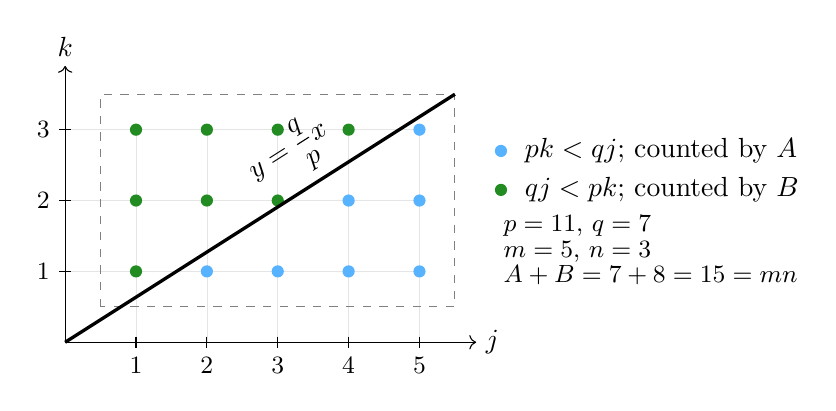
\begin{tikzpicture}[x=0.9cm,y=0.9cm]
    \draw[step=0.9cm,gray!20,very thin] (0,0) grid (5,3);
    \draw[->] (0,0) -- (5.8,0) node[right] {$j$};
    \draw[->] (0,0) -- (0,3.9) node[above] {$k$};
    \draw[dashed,gray] (0.5,0.5) rectangle (5.5,3.5);

    \foreach \j in {1,...,5}
        \draw (\j,0.08) -- (\j,-0.08) node[below] {\small $\j$};
    \foreach \k in {1,...,3}
        \draw (0.08,\k) -- (-0.08,\k) node[left] {\small $\k$};

    \foreach \point in {(2,1),(3,1),(4,1),(4,2),(5,1),(5,2),(5,3)}
        \fill[brandblue] \point circle (2.2pt);
    \foreach \point in {(1,1),(1,2),(1,3),(2,2),(2,3),(3,2),(3,3),(4,3)}
        \fill[ForestGreen] \point circle (2.2pt);

    \draw[very thick] (0,0) -- (5.5,3.5)
        node[pos=0.63,above,sloped] {$y=\dfrac{q}{p}x$};

    \fill[brandblue] (6.15,2.7) circle (2.2pt);
    \node[anchor=west] at (6.35,2.7) {$pk<qj$; counted by $A$};
    \fill[ForestGreen] (6.15,2.15) circle (2.2pt);
    \node[anchor=west] at (6.35,2.15) {$qj<pk$; counted by $B$};
    \node[anchor=west,align=left] at (6.05,1.3)
        {\small $p=11$, $q=7$\\[-1mm]
         \small $m=5$, $n=3$\\[-1mm]
         \small $A+B=7+8=15=mn$};
\end{tikzpicture}

\textit{The case $p=11$ and $q=7$: each of the $mn=15$ lattice
points lies strictly below or strictly above the line.}
\end{center}

The sum $A$ counts the points for which $pk<qj$, while $B$ counts
the points for which $qj<pk$. Equality cannot occur: if $pk=qj$,
then the distinct primes $p$ and $q$ would force $p\mid j$, which is
impossible because $1\leq j<p$. Hence every point is counted exactly
once by either $A$ or $B$, and therefore
\[
    A+B=mn=\frac{p-1}{2}.\frac{q-1}{2}
    \]
Consequently,
\[
    \left(\frac pq\right)\left(\frac qp\right)
      =(-1)^{A+B}
      =(-1)^{\frac{p-1}{2}.\frac{q-1}{2}},
\]
which proves the law.
\hfill$\square$
\end{claim_box}

\begin{remark_box}
\textbf{Lemma:}
Let $p$ and $q$ be distinct odd primes. Then
\[
    \boxed{\left(\frac pq\right)=-\left(\frac qp\right)}
\]
if and only if
\[
    p\equiv q\equiv3\pmod4.
\]
Equivalently, this occurs exactly when
$p=4k+3$ and $q=4\ell+3$ for some nonnegative integers $k,\ell$.
\end{remark_box}

\begin{claim_box}
\textit{Proof:}
Since $p$ and $q$ are distinct primes, both Legendre symbols are in
$\{-1,1\}$. Therefore
\[
    \left(\frac pq\right)=-\left(\frac qp\right)
\]
holds exactly when
\[
    \left(\frac pq\right)\left(\frac qp\right)=-1.
\]
By quadratic reciprocity,
\[
    \left(\frac pq\right)\left(\frac qp\right)
      =(-1)^{\frac{p-1}{2}\cdot\frac{q-1}{2}}.
\]
This sign is $-1$ exactly when
\[
    \frac{p-1}{2}\cdot\frac{q-1}{2}
\]
is odd. A product of integers is odd if and only if both factors are
odd. For an odd prime $r$,
\[
    \frac{r-1}{2}\text{ is odd}
      \quad\Longleftrightarrow\quad r\equiv3\pmod4.
\]
Hence the two Legendre symbols have opposite signs if and only if
$p\equiv q\equiv3\pmod4$.
\hfill$\square$
\end{claim_box}

\begin{example_box}
For example, quadratic reciprocity gives
\[
    \left(\frac{3}{11}\right)
      =-\left(\frac{11}{3}\right)
      =-\left(\frac{2}{3}\right)=1.
\]
Indeed, $5^2=25\equiv3\pmod{11}$.
\end{example_box}

\textbf{Note:} This law is extremely powerful in the sense that we can now find $(\frac{p}{q})$ for any odd primes $p,q$ because their gcd is bound to be 1, and we can keep applying the euclidean division algorithm by reversing the numerator and denominator until we reach $1$, and we know that $(\frac{1}{r})=1$ for any $r$, as $1=1^2$ thus it is trivially a quadratic residue for any $r$. Thus we can extend it to all natural numbers $n,m$ as they can be factorised into primes. So it is possible to find out $(\frac{n}{m})$ for any $n,m$.

\begin{example_box}
For example,
\begin{align*}
    \left(\frac{29}{43}\right)
      &=\left(\frac{43}{29}\right)
       =\left(\frac{14}{29}\right)\\
      &=\left(\frac{2}{29}\right)
        \left(\frac{7}{29}\right)
       =(-1)\left(\frac{29}{7}\right)
       =-\left(\frac17\right)=-1.
\end{align*}
Thus $29$ is a quadratic nonresidue modulo $43$.
\end{example_box}

\section{The Jacobi Symbol}

The Legendre symbol is defined only when the denominator is prime.
The Jacobi symbol extends this notation to every positive odd
denominator by using its prime factorization. It preserves the
algebraic rules and reciprocity laws of the Legendre symbol, making it
possible to perform computations without first factoring the
denominator completely. However, one important distinction must be
kept in mind: a Jacobi symbol equal to $1$ does not necessarily mean
that the numerator is a quadratic residue modulo the denominator.

\subsection{Definition and Basic Properties}

\begin{definition_box}
Let $n$ be a positive odd integer with prime factorization
\[
    n=p_1^{\alpha_1}\cdots p_r^{\alpha_r}.
\]
For any integer $a$, the \emph{Jacobi symbol} is defined by
\[
    \left(\frac an\right)
      :=\prod_{i=1}^{r}
        \left(\frac{a}{p_i}\right)^{\alpha_i},
\]
where each factor on the right is a Legendre symbol. We also define
\[
    \left(\frac a1\right)=1.
\]
\end{definition_box}

\begin{example_box}
Since $45=3^2\cdot5$,
\[
    \left(\frac{7}{45}\right)
      =\left(\frac73\right)^2\left(\frac75\right)
      =1\cdot\left(\frac25\right)=-1.
\]
\end{example_box}

\begin{mainbox}{Basic properties of the Jacobi symbol:}
Let $m,n$ be positive odd integers and let $a,b\in\mathbb{Z}$. Then:
\begin{enumerate}
    \item $\left(\frac an\right)\in\{-1,0,1\}$, and
    \[
        \left(\frac an\right)=0
          \quad\Longleftrightarrow\quad \gcd(a,n)>1.
    \]
    \item If $a\equiv b\pmod n$, then
    \[
        \left(\frac an\right)=\left(\frac bn\right).
    \]
    \item The symbol is multiplicative in the numerator:
    \[
        \left(\frac{ab}{n}\right)
          =\left(\frac an\right)\left(\frac bn\right).
    \]
    \item The symbol is multiplicative in the denominator:
    \[
        \left(\frac{a}{mn}\right)
          =\left(\frac am\right)\left(\frac an\right).
    \]
\end{enumerate}
\end{mainbox}

\subsection{Supplementary Laws}

\begin{remark_box}
\textbf{Parity lemma:}
Let
\[
    N=p_1^{\alpha_1}\cdots p_r^{\alpha_r}
\]
be a positive odd integer. Then
\[
    \sum_{i=1}^{r}\alpha_i\frac{p_i-1}{2}
      \equiv\frac{N-1}{2}\pmod2,
\]
and
\[
    \sum_{i=1}^{r}\alpha_i\frac{p_i^2-1}{8}
      \equiv\frac{N^2-1}{8}\pmod2.
\]
\end{remark_box}

\begin{claim_box}
\textit{Proof:}
For any positive odd integers $u$ and $v$,
\[
    \frac{uv-1}{2}
      =\frac{u-1}{2}+\frac{v-1}{2}
       +\frac{(u-1)(v-1)}{2}.
\]
Since $u-1$ and $v-1$ are both even, their product is divisible by
$4$. Hence the final term is even, and therefore
\[
    \frac{uv-1}{2}
      \equiv\frac{u-1}{2}+\frac{v-1}{2}\pmod2.
\]
Applying this congruence repeatedly to the prime factors of $N$,
counted with multiplicity, gives
\[
    \frac{N-1}{2}
      \equiv\sum_{i=1}^{r}\alpha_i\frac{p_i-1}{2} \pmod2.
\]

Similarly,
\[
    \frac{u^2v^2-1}{8}
      =\frac{u^2-1}{8}+\frac{v^2-1}{8}
       +\frac{(u^2-1)(v^2-1)}{8}.
\]
The square of every odd integer is congruent to $1$ modulo $8$, so
both $u^2-1$ and $v^2-1$ are divisible by $8$. The final term is
therefore even, and
\[
    \frac{u^2v^2-1}{8}
      \equiv\frac{u^2-1}{8}+\frac{v^2-1}{8}\pmod2.
\]
Repeating this over the prime factors of $N$ proves the second
congruence.
\hfill$\square$
\end{claim_box}

\begin{mainbox}{Supplementary laws for the Jacobi symbol:}
For every positive odd integer $n$,
\[
    \left(\frac{-1}{n}\right)=(-1)^{(n-1)/2}
      =
      \begin{cases}
          1 & \text{if $n\equiv1\pmod4$},\\
         -1 & \text{if $n\equiv3\pmod4$},
      \end{cases}
\]
and
\[
    \left(\frac2n\right)=(-1)^{(n^2-1)/8}
      =
      \begin{cases}
          1 & \text{if $n\equiv1$ or $7\pmod8$},\\
         -1 & \text{if $n\equiv3$ or $5\pmod8$}.
      \end{cases}
\]
\end{mainbox}

\begin{claim_box}
\textit{Proof:}
Write
\[
    n=p_1^{\alpha_1}\cdots p_r^{\alpha_r}.
\]
Using the definition of the Jacobi symbol and the first supplementary
law for Legendre symbols, we obtain
\begin{align*}
    \left(\frac{-1}{n}\right)
      &=\prod_{i=1}^{r}
        \left(\frac{-1}{p_i}\right)^{\alpha_i}\\
      &=\prod_{i=1}^{r}
        (-1)^{\alpha_i(p_i-1)/2}\\
      &=(-1)^{\sum_{i=1}^{r}
        \alpha_i(p_i-1)/2}.
\end{align*}
The parity lemma gives
\[
    \sum_{i=1}^{r}\alpha_i\frac{p_i-1}{2}
      \equiv\frac{n-1}{2}\pmod2,
\]
and hence
\[
    \left(\frac{-1}{n}\right)=(-1)^{(n-1)/2}.
\]

Likewise, the second supplementary law for Legendre symbols gives
\begin{align*}
    \left(\frac2n\right)
      &=\prod_{i=1}^{r}
        \left(\frac2{p_i}\right)^{\alpha_i}\\
      &=(-1)^{\sum_{i=1}^{r}
        \alpha_i(p_i^2-1)/8}.
\end{align*}
By the second congruence in the parity lemma,
\[
    \sum_{i=1}^{r}\alpha_i\frac{p_i^2-1}{8}
      \equiv\frac{n^2-1}{8}\pmod2,
\]
so
\[
    \left(\frac2n\right)=(-1)^{(n^2-1)/8}.
\]
The stated residue-class descriptions follow immediately by checking
the odd classes modulo $4$ and modulo $8$.
\hfill$\square$
\end{claim_box}

\subsection{Quadratic Reciprocity for Jacobi Symbols}

\begin{mainbox}{General law of quadratic reciprocity:}
Let $m$ and $n$ be coprime positive odd integers. Then
\[
    \left(\frac mn\right)\left(\frac nm\right)
      =(-1)^{\frac{m-1}{2}\cdot\frac{n-1}{2}}.
\]
Equivalently,
\[
    \left(\frac mn\right)=\left(\frac nm\right)
\]
unless $m\equiv n\equiv3\pmod4$, in which case
\[
    \left(\frac mn\right)=-\left(\frac nm\right).
\]
\end{mainbox}

\begin{claim_box}
\textit{Proof:}
Write
\[
    m=\prod_{i=1}^{r}p_i^{\alpha_i},
    \qquad
    n=\prod_{j=1}^{s}q_j^{\beta_j}.
\]
Since $\gcd(m,n)=1$, no $p_i$ equals any $q_j$. By multiplicativity
and prime quadratic reciprocity,
\begin{align*}
    \left(\frac mn\right)\left(\frac nm\right)
      &=\prod_{i=1}^{r}\prod_{j=1}^{s}
        \left[
          \left(\frac{p_i}{q_j}\right)
          \left(\frac{q_j}{p_i}\right)
        \right]^{\alpha_i\beta_j}\\
      &=(-1)^E,
\end{align*}
where
\[
    E=\left(\sum_{i=1}^{r}
       \alpha_i\frac{p_i-1}{2}\right)
      \left(\sum_{j=1}^{s}
       \beta_j\frac{q_j-1}{2}\right).
\]
By the parity lemma,
\[
    \sum_i\alpha_i\frac{p_i-1}{2}
      \equiv\frac{m-1}{2}\pmod2.
\]
Similarly,
\[
    \sum_j\beta_j\frac{q_j-1}{2}
      \equiv\frac{n-1}{2}\pmod2.
\]
Therefore
\[
    E\equiv\frac{m-1}{2}\cdot\frac{n-1}{2}\pmod2,
\]
which proves the formula.
\hfill$\square$
\end{claim_box}

\begin{example_box}
For example,
\begin{align*}
    \left(\frac{73}{95}\right)
      &=\left(\frac{95}{73}\right)
       =\left(\frac{22}{73}\right)\\
      &=\left(\frac2{73}\right)
        \left(\frac{11}{73}\right)
       =\left(\frac{73}{11}\right)\\
      &=\left(\frac7{11}\right)
       =-\left(\frac{11}{7}\right)
       =-\left(\frac47\right)=-1.
\end{align*}
Here $\left(\frac2{73}\right)=1$ because $73\equiv1\pmod8$.
\end{example_box}

\subsection{Relation to Quadratic Residues}

\begin{remark_box}
Let $n$ be a positive odd integer and suppose $\gcd(a,n)=1$. If $a$
is a quadratic residue modulo $n$, then
\[
    \left(\frac an\right)=1.
\]
The converse is generally false when $n$ is composite.
\end{remark_box}

\begin{claim_box}
\textit{Proof:}
If $x^2\equiv a\pmod n$, then for every prime $p\mid n$ we also have
\[
    x^2\equiv a\pmod p.
\]
Thus $a$ is a nonzero quadratic residue modulo every prime divisor of
$n$, so every Legendre symbol occurring in the definition of the
Jacobi symbol equals $1$. Hence
\[
    \left(\frac an\right)=1.
\]
\hfill$\square$
\end{claim_box}

\begin{example_box}
The converse fails for composite denominators. Indeed,
\[
    \left(\frac2{15}\right)
      =\left(\frac23\right)\left(\frac25\right)
      =(-1)(-1)=1.
\]
Nevertheless, $2$ is not a quadratic residue modulo $15$, since a
solution of $x^2\equiv2\pmod{15}$ would give
$x^2\equiv2\pmod3$, which is impossible.
\end{example_box}

\end{document}
